%-----------------------------------------------------------------------------
%
%               Template for sigplanconf LaTeX Class
%
% Name:         sigplanconf-template.tex
%
% Purpose:      A template for sigplanconf.cls, which is a LaTeX 2e class
%               file for SIGPLAN conference proceedings.
%
% Author:       Paul C. Anagnostopoulos
%               Windfall Software
%               978 371-2316for the
%               paul@windfall.com
%
% Created:      15 February 2005
%
%-----------------------------------------------------------------------------


\documentclass{sigplanconf}  %[preprint]

% The following \documentclass options may be useful:
%
% 10pt          To set in 10-point type instead of 9-point.
% 11pt          To set in 11-point type instead of 9-point.
% authoryear    To obtain author/year citation style instead of numeric.

\usepackage{amsmath}
\usepackage{amssymb}
\usepackage{amsthm}

\usepackage{multicol}
\usepackage{multirow}
\usepackage{graphicx}
\usepackage{color}
\usepackage{subfigure}
\usepackage{epsfig}
\usepackage{fancybox}
\usepackage{fancyvrb}

\usepackage{amssymb}
\usepackage{amsthm}

\usepackage{rotating}

\usepackage{hyperref} % comes last, as it redefines a couple of commands
\hypersetup{
    colorlinks,%
    citecolor=black,%
    filecolor=black,%
    linkcolor=black,%
    urlcolor=blue
}

\DefineVerbatimEnvironment{colorcode}%
        {Verbatim}{fontsize=\small,commandchars=\\\{\}}   % \normalsize
        %{Verbatim}{fontsize=\scriptsize,commandchars=\\\{\}}


\definecolor{DikuRed}{RGB}{130,50,32}
\newcommand{\emp}[1]{\textcolor{DikuRed}{ #1}}
\definecolor{CosGreen}{RGB}{10,100,70}
\newcommand{\emphh}[1]{\textcolor{CosGreen}{ #1}}


\newcommand{\mymath}[1]{$ #1 $}
\newcommand{\myindx}[1]{_{#1}}
\newcommand{\myindu}[1]{^{#1}}
\newcommand{\mymathbb}[1]{\mathbb{#1}}

\hyphenation{ho-mo-mor-phism}
\hyphenation{list-ho-mo-mor-phism}
\hyphenation{mul-ti-pli-ca-tion}
\hyphenation{re-le-vant}
\hyphenation{asso-ci-a-ti-vi-ty}

\renewcommand\tilde[0]{{\raise.17ex\hbox{$\scriptstyle\sim$}}}
\newcommand{\LO}{$\mathcal{L}_0$}

%%%%%%%%%%%%%%%%%%%%%%%
% comments
\usepackage{color}
\newcommand{\comment}[2]{\textcolor{red}{\scriptsize \textsf \textbf{#1:}{#2}}}

% to switch comments off, activate this definition
% \renewcommand{\comment}[2]{}

%%%%%%%%%%%%%%%%%%%%%%%

\begin{document}

\conferenceinfo{FHPC'13,} {September 23, 2013, Boston, Massachusets.}
\CopyrightYear{2013}
%\copyrightdata{978-1-4503-1577-7/12/09}


\title{A Structural-Analysis Approach To Fusion}
\subtitle{\LO{} Status Report}
%\subtitle{Subtitle Text, if any}

%%%%%%%%%%%%%%%%%%%
%%% AUTHORS INF %%%
%%%%%%%%%%%%%%%%%%%

\authorinfo{Troels Henriksen, Cosmin E. Oancea}
           {HIPERFIT, Department of Computer Science, University of Copenhagen (DIKU)}
           {cosmin.oancea@diku.dk, athas@sigkill.dk}


%%%%%%%%%%%%%%%%%%%
%%%%%%%%%%%%%%%%%%%
%%%%%%%%%%%%%%%%%%%

\maketitle
%\renewcommand{\comment}[2]{}



\begin{abstract}

Fusion is one of the most important code transformations as it 
has the potential to substantially optimize both the memory hierarchy 
time overhead and (sometimes asymptotically) the space requirement.
%
In imperative languages, the legality of loop-fusion is typically 
verified by dependency analysis on arrays applied at loop-nest level.
Such analysis, however, has often been labeled as ``heroic effort''
and, if at all, is supported only in its simplest and most
conservative form in industrial compilers.  

In functional languages, fusion is naturally and more easily derived
as a producer-consumer relation between program constructs that expose
a richer, higher-order algebra of program invariants, 
%from the richer, higher-order semantics of program invariants, 
such as the {\tt map-reduce} list homomorphisms. %algebra.   

Related implementations in the functional context typically 
apply fusion only when the to-be-fused producer is used exactly once,
i.e., in the consumer.   This guarantees that the transformation is
conservative: the resulting program does not duplicate computation.

We show that the above restriction is more conservative than needed,
and present a structural-analysis algorithm, inspired
from the {\tt T$_1$-T$_2$} transformation for reducible data flow,
that enables fusion even in some cases when the producer is used 
in different consumers {\em and} without duplicating computation.  

We report an implementation of the fusion algorithm for a 
{\em functional}-core language, named \LO{}, which is intended 
to support {\em nested} parallelism across {\em regular} 
multi-dimensional arrays.  We succinctly describe \LO's
semantics and the compiler infrastructure on which the fusion
transformation relies.

\end{abstract}

%\category{CR-number}{subcategory}{third-level}
\category{D.1.3}{Concurrent Programming}{Parallel Programming}
%\category{D.1.3}{Programming Techniques}{Concurrent Programming}%%[Parallel Programming]
\category{D.3.4}{Processors}{Compiler}


\terms
Performance, Design, Algorithms

\keywords
fusion, autoparallelization, functional language

\section{Introduction}
\label{sec:Introduction}

%%%%%%%%%%%%%%%%%%%%%%%%%%%%%%%%%%%%%%%%%%%%%%%%%%%%%%%%%%%%%%
%%% HL Introduction: financial motivation + GPU motivation %%%
%%% + our generic-pricing case study + short description   %%%
%%%%%%%%%%%%%%%%%%%%%%%%%%%%%%%%%%%%%%%%%%%%%%%%%%%%%%%%%%%%%%

%The motivation for the $\mathcal{L}_0$ language steams from
%one of the goals of the {\sc hiperfit} project

One of the main goals of the {\sc hiperfit} project has been to
develop the infrastructure necessary to write real-world, big-data 
financial applications in a hardware-independent language that can 
be efficiently executed on massively parallel hardware, e.g., {\sc gpgpu}.  % various 

In this sense we have examined several such computational kernels~\cite{PricingFHPC}, 
originally implemented in languages such as OCaml, Python, C++, C
and measuring in the range of hundreds/thousands lines of compact code, 
with two main objectives in mind: 
\begin{itemize}
    \item[1.] What should be a suitable core language that, on the
                one hand, would allow a relatively straight-forward 
                code translation, and, on the other hand, would
                preserve the algorithmic invariants that are needed
                to optimize the application globally?
    \item[2.] What compiler optimizations would result in efficiencies
                comparable to the hardware hand-tuned version 
                of the code?
\end{itemize}

The answer to the first question has been %, not surprisingly, 
a {\em functional} language, dubbed \LO{}, supporting %with support for 
\texttt{map-reduce} {\em nested} parallelism on {\em regular} arrays, i.e., 
the size of each dimension is constant at runtime:\\
It is {\em regular} because our suite does not require irregular 
arrays in the sense of {\sc nesl} or {\sc dph}~\cite{BlellochCACM96NESL,Chak06DPH}, 
and regular arrays are more amenable to compiler optimizations.
%
It is {\em nested} because our suite exhibits several layers of 
parallelism that cannot be exploited by flat parallelism in the style of 
{\sc repa}~\cite{REPA}, e.g., several innermost {\tt scan} or 
{\tt reduce} operations and at least one (semantically)
sequential loop per benchmark.
%
Finally, it is {\em functional} because we would rather invest compiler effort
in exploiting high-level program invariants rather than in proving them.
The common example here is parallelism: {\tt map-reduce} 
constructs are inherently parallel, while Fortran-style \texttt{do} 
loops require sophisticated analysis to decide parallelism. 
Furthermore, such analyses~\cite{Blume94RangeTest,SUIF,CosPLDI} %there is solid evidence that such 
have not yet been integrated in the repertoire of commercial compilers,
likely due to ``heroic effort'' concerns, albeit
 (i) their effectiveness was demonstrated on comprehensive suites, and
(ii) some of them were developed more than a decade ago.

Perhaps less expectedly, the answer to the second question seems to be 
that a common ground needs to be found between functional and imperative
optimizations and, to a less extent,  between language constructs.
Much in the same way in which (data) parallelism seems to be generated by
a combination of {\tt map}, {\tt reduce}, and {\tt scan} operations, 
the optimization opportunities, e.g., enhancing the degree of parallelism 
and reducing  the memory time and space overheads, seem solvable via a 
combination of {\tt fusion}, {\tt transposition}, loop {\tt interchange} 
and {\tt distribution}~\cite{OptCompModernArch}.
%
It follows that loops are necessary in the intermediate representation,
regardless of whether they are provided as a language construct or are
derived from tail-recursive functions via a code transformation. 

Finally, an indirect consequence of having to deal with sequential (dependent) 
%, which semantically update an unknown array index at a time, 
loops is that \LO{} provides support for ``in-place updates'' of 
array elements. The semantics is the functional one, i.e., %the result is a
deep copy of the original array but with the corresponding element replaced,
\texttt{intersected} with the imperative one, i.e., if aliasing may prevent 
an in-place implementation a compile-time error is signaled.   The approach
enables a (optimized) cost model that the user likely assumes, while 
preserving the functional semantics. 
%allows both a functional semantics and the cost model that the user likely assumes.

Section~\ref{sec:Prelim} provides an overview of the \LO{} language % brief 
and of the enabling optimizations that set the stage for fusion. %'s application.% transformation.

%\footnote{
%The reasons are that our current benchmark does not require irregular arrays in 
%the sense of {\sc nesl}~\cite{BlellochCACM96NESL}, and regular arrays are more
%amenable to compiler optimizations.
%}    
%L$0$ is a first-order functional core-language intended to support nested 
%parallelism across regular multi-dimensional arrays, 
%%%, i.e., sizes of each array dimension match,
%by means of the typical set of second-order array combinators such
%as \texttt{map}, \texttt{reduce}, \texttt{scan}, \texttt{filter}, \texttt{zip}, etc.





%In the remainder of this section we provide a rationale for our case study and an overview
%of the optimization techniques evaluated.  In the following sections we present the functional
%formulation of the pricing algorithm (Section~\ref{sec:AlgLang}), the optimizations for
%compiling it to {\tt OpenCL} (Section~\ref{sec:Optimizations}), the empirical evaluation of the
%optimizations' impact (Section~\ref{sec:ExpRes}),
%a review of related work on imperative and functional parallelization (Section~\ref{sec:RelWork}),
%and finally our conclusions as to what has been accomplished so far and which future work this suggests
%(Section~\ref{sec:Concl}).

\section{Preliminaries: $\mathcal{L}_0$ and Enabling Optimizations}
\label{sec:Prelim}

For Troels:
\begin{itemize}
    \item[1.] Figure with language grammar or \textsc{AbSyn} $+$ brief explanations.
    \item[2.] One or more seducing code examples with loops and in-place updates (may I suggest TRIDAG?) 
                $+$ brief explanation of loop semantics (equivalence to tail-recursive function) $+$
    \item[3.] in-place update semantics and checking (uniqueness types, aliasing analysis)
    \item[4.] Figure with enabling optimizations $+$ brief explanation for each.
    \item[5.] Demonstration of how code looks like after tuple-of-array transformation,
                i.e., that would be the input for fusion.
\end{itemize}

\LO{} is a mostly-monomorphic, statically typed, strictly evaluated,
purely functional language.  Although some built-in higher-order
functions provide polymorphism, user-defined functions are
monomorphic, and their return- and parameter types must be specified
explicitly.  For brevity, we will not cover the typing
rules in detail, as they are quite trivial.  The only exception is our
notion of {\em uniqueness types}, which is given a cursory treatment
in Section~\ref{sec:in-place}.

The syntax of the first-order fragment of \LO{} can be seen in Figure~\ref{fig:fo-syntax}.  
Common arithmetic operators such as {\tt +} and
{\tt /} are supported in the usual way.  Note that they are
polymorphic in the sense that they accept both integers and
floating-points, although both operands must be of the same type.
Pattern matching is supported in a limited way as the only way of
decomposing tuple values, but there is no {\tt case} construct.  
Note that braces denote arrays, not sets.

{\tt zip} and {\tt unzip} behave as usual, i.e, {\tt
  zip(\{1,2,3\},\{4,5,6\})} $=$ {\tt \{{(1,4),(2,5),(3,6)}\}}, but the
semantics of {\tt zip} requires that the input arrays have outermost
dimensions of equal sizes. Otherwise a compile or runtime error is signalled.
%It is an error if the arrays given to {\tt zip} are not of the exact same size.

There are two non-standard constructs in the first-order part  % slightly complicated
of \LO{}.  The first is the let-with construct for updating parts of
arrays:

\begin{colorcode}
let b = a with [i\mymath{\myindx{1}},..,i\mymath{\myindx{k}}] <- v in body
\end{colorcode}

The above evaluates {\tt body} with {\tt b} bound to the value of {\tt a}, 
except that the element at position {\tt (i$_1$,..,i$_k$)} is updated to
the value of {\tt v}.  If {\tt a[i$_1$,..,i$_k$]} is itself an array,
i.e., if {\tt a} has more than {\tt k} dimensions, {\tt v} must be 
%(that is, if {\tt a} has more than {\tt k} dimensions), {\tt v} must be 
an array of the same size as the slice it is replacing.  We write 
{\tt let~a[i$_1$,..,i$_k$]~=~v~in~body} when the 
source and destination array share the same name.
%variable to be bound has the same name as the source variable.  
%
Section~\ref{sec:in-place} describes our method for doing array updates 
{\em in-place} without losing referential transparency. This allows a 
cost model in which the update takes time proportional to the total 
size of {\tt v}, rather~than~{\tt a}.

The other non-standard construct is the {\tt do}-loop:  
It is fundamentally syntactical sugar for a certain form of 
tail-recursive function, and is used by the user to express
certain sequential computation that would be awkward to write
functionally, and by the compiler in lower-level optimisations,
such as loop interchange, distribution.  

%The other unusual construct is the {\tt do}-loop:  
%It is fundamentally
%syntactical sugar for a certain form of tail-recursive function, 
%in order to make it easier to express loop optimisations and certain
%sequential loops.

For example, denoting by {\tt t} the type of {\tt x}, the loop in
Figure~\ref{fig:loop-recursion} has the semantics of a call to the
recursive function on the right-hand side.

\begin{figure}
\begin{minipage}{0.35\columnwidth}
\begin{colorcode}
loop (x = a) =
  for i < n do
    g(x)
in body
\end{colorcode}
\end{minipage}
\begin{minipage}{0.05\columnwidth}
$\Rightarrow$
\end{minipage}
\begin{minipage}{0.6\columnwidth}
\begin{colorcode}
fun t f(int i, int n, t x) =
  if i >= n then x
     else f(i+1, n, g(x))

let x = f(i, n, a)
in body
\end{colorcode}
\end{minipage}
\caption{Loop to recursive function}
\label{fig:loop-recursion}
\end{figure}

\begin{figure}[bt]
\begin{tabular}{lrll}
$t$ & $::=$ & {\tt int} & (Integers) \\
& $|$ & {\tt real} & (Floats) \\
& $|$ & {\tt bool} & (Booleans) \\
& $|$ & {\tt char} & (Characters) \\
& $|$ & {\tt ($t_{1}$, \ldots, $t_{n}$)} & (Tuples) \\
& $|$ & {\tt [$t$]} & (Arrays) \\
\\
$v$ & $::=$ & $k$ & (Integer)\\
& $|$ & $x$ & (Decimal number) \\
& $|$ & $b$ & (Boolean)\\
& $|$ & $c$ & (Character)\\
& $|$ & $(v_{1},\ldots,v_{n})$ & (Tuple) \\
& $|$ & $\{v_{1},\ldots,v_{n}\}$ & (Array) \\
\\
$p$ & $::=$ & {\tt {\bf id}} & (Name pattern)\\
& $|$ & {\tt ($p_{1}$, \ldots, $p_{n}$)} & (Tuple pattern) \\
\\
$e$ & $::=$ & $v$ & (Constant)\\
& $|$ & ${\bf id}$ & (Variable)\\
& $|$ & {\tt ($e_{1}$,\ldots,$e_{n}$)} & (Tuple expression) \\
& $|$ & {\tt \{$e_{1}$,\ldots,$e_{n}$\}} & (Array expression) \\
& $|$ & $e_{1} \odot{} e_{2}$ & (Binary operator) \\
& $|$ & {\tt \tilde{} $e$} & (Prefix minus) \\
& $|$ & {\tt not $e$} & (Logical negation) \\
& $|$ & {\tt if $e_{1}$ then $e_{2}$ else $e_{3}$} & (Branching) \\
& $|$ & {\tt {\bf id}[$e_{1}$, \ldots, $e_{n}$]} & (Indexing) \\
& $|$ & {\tt {\bf id}($e_{1}$, \ldots, $e_{n}$)} & (Function call) \\
& $|$ & {\tt let $p$ = $e_{1}$ in $e_{2}$} & (Pattern binding) \\
& $|$ & {\tt zip($e_{1}$, \ldots, $e_{n}$)} & (Zipping) \\
& $|$ & {\tt unzip($e$)} & (Unzipping) \\
& $|$ & {\tt iota($e$)} & (Range) \\
& $|$ & {\tt replicate($e_{n}$, $e_{v}$)} & (Replication) \\
& $|$ & {\tt size($e$)} & (Array length) \\
& $|$ & {\tt transpose($e$)} & (Transposition) \\
& $|$ & {\tt split($e_{1}$, $e_{2}$)} & (Split $e_{2}$ at index $e_{1}$) \\
& $|$ & {\tt concat($e_{1}$, $e_{2}$)} & (Concatenation) \\
& $|$ & {\tt let $\alpha$ = $\beta$ with} & (In-place update) \\
&     & {\tt \ \ [$e_{1}$,\ldots,$e_{n}$] <- $e_{v}$} \\
&     & {\tt in $e_{b}$} \\
& $|$ & {\tt loop ($p$ = $e_{1}$) =} & (Loop) \\
&     & {\tt \ \ for $\alpha$ < $e_{2}$ do $e_{3}$} \\
&     & {\tt in $e_{4}$} \\
\end{tabular}
\\
\begin{tabular}{lrll}
$fun$ & $::=$ & {\tt fun $t$ {\bf id}($t_{1}$ {\bf id}$_{1}$,\ldots $t_{n}$ {\bf id}$_{n}$) = $e$} \\
\\
$prog$ & $::=$ & $\epsilon$ \\
       & $|$   & $fun$ $prog$
\end{tabular}
\caption{\LO{} syntax}
\label{fig:fo-syntax}
\end{figure}

\subsection{Second-order array combinators}
\label{sec:soacs}

Most array operations in \LO{} are done through built-in second-order
array combinators ({\sc soac}s).  The available {\sc soac}s can be seen in Figure
\ref{fig:soacs}, along with our syntax for anonymous and curried
functions.  As \LO{} is first-order, these anonymous functions are
only syntactically permitted in {\sc soac} invocations.  The parentheses may
be omitted when currying if no curried arguments are given.

\begin{figure}[bt]
\begin{tabular}{lrll}
$l$ & $::=$ & {\tt fn $t$ ($t_{1}$ {\bf id}$_{1}$, \ldots, $t_{n}$ {\bf id}$_{n}$)} & (Anonymous function) \\
&     & {\tt => $e$} \\
& $|$ & {\tt {\bf id} ($e_{1}$, \ldots, $e_{n}$)} & (Curried function) \\
& $|$ & {\tt op $\odot$ ($e_{1}$, \ldots, $e_{n}$)} & (Curried operator) \\
\\
$e$ & $::=$ & {\tt map($l$, $e$)} \\
    & $|$ & {\tt filter($l$, $e$)} \\
    & $|$ & {\tt reduce($l$, $x$, $e$)} \\
    & $|$ & {\tt scan($l$, $x$, $e$)} \\
    & $|$ & {\tt redomap($l_{r}$, $l_{m}$, $x$, $e$)} \\
\end{tabular}
\caption{Second-order array combinators}
\label{fig:soacs}
\end{figure}

The semantics of the {\sc soac}s is identical to the similarly-named
higher-order functions found in many functional languages, but we
reproduce it here for completeness.  Note the types given are not \LO{}
types, but a Haskell-inspired notation, since the {\sc soac}s cannot be 
typed in \LO{} itself.
\begin{align*}
\text{\tt map($f$,$a$)}
& :: (\alpha\rightarrow\beta)\rightarrow[\alpha]\rightarrow[\beta] \\
& \equiv \text{\tt\{$f$($a$[0]), \ldots, $f$($a$[n])\}}
\end{align*}
\begin{align*}
\text{\tt filter}
& :: (\alpha\rightarrow{\tt bool})\rightarrow[\alpha]\rightarrow[\alpha] \\
\text{\tt filter($f$,a)} & \equiv \text{\tt\{$a$[i] | $f$($a$[i]) = {\tt True }\}}
\end{align*}
\begin{align*}
\text{\tt reduce}
& :: (\alpha\rightarrow\alpha\rightarrow\alpha)\rightarrow\alpha\rightarrow[\alpha]\rightarrow\alpha \\
\text{\tt reduce($f$,$x$,$a$)} & \equiv \text{\tt $f$($f$(\ldots $f$($x$,$v$[0]), $v$[1]), $v$[n])}
\end{align*}
\begin{align*}
\text{\tt scan}
& :: (\alpha\rightarrow\alpha\rightarrow\alpha)\rightarrow\alpha\rightarrow[\alpha]\rightarrow[\alpha] \\
\text{\tt scan($f$,$x$,a)} & \equiv \text{\tt\{$f$($x$,$a$[0]), $f$($f$($x$,$a$[0]),$v$[1]),\ldots\}}
\end{align*}

In particular, note that {\tt scan} is an inclusive prefix scan.  {\tt
  redomap} is a special case -- it is not part of the external \LO{}
language, but used internally for fusing {\tt reduce} and {\tt map}.
Its semantics is as follows.
\begin{align*}
\text{\tt redomap}
& :: (\alpha\rightarrow\alpha\rightarrow\alpha)\rightarrow(\alpha\rightarrow\beta\rightarrow\alpha)\\
& \quad\rightarrow\alpha\rightarrow[\beta]\rightarrow\alpha \\
\text{\tt redomap($f$,$g$,$x$,$v$)} & \equiv \text{\tt foldl($g$, $x$, $v$)}
\end{align*}
Note that the runtime semantics is a left-fold, not a normal \LO{}
\texttt{reduce}.  The rationale behind {\tt redomap} is as follows;
using a Haskell-like syntax.

{\tt (red $\odot$ e) . (map f)} can be formally transformed, via the
list homomorphism ({\sc lh}) promotion lemma~\cite{BirdListTh}, to an
equivalent form:  \\
${\tt red}\mbox{ }\odot\mbox{ }{\tt e}\mbox{ }.\mbox{ }{\tt map}\mbox{
}{\tt f}\mbox{ }\emphh{\equiv}$ $\mbox{ }{\tt red}\mbox{ }\odot\mbox{
}{\tt e}\mbox{ }.\mbox{ }{\tt pmap}_{p} \mbox{ }$ $(\emp{{\tt red} \mbox{
  }\odot\mbox{ }{\tt e}\mbox{ }.\mbox{ }{\tt map}\mbox{ }{\tt f}})$\\
where the original list is distributed to $p$ parallel processors,
each of which execute the original map-reduce computation sequentially
and, at the end, reduce in parallel the per-processor result.  Hence
the {\em inner} map-reduce can be
rewritten as a left-fold:\\
${\tt red}\mbox{ }\odot\mbox{ }{\tt e}\mbox{ }.\mbox{ }{\tt map}\mbox{
}{\tt f}\mbox{ }\emphh{\equiv}$ $\mbox{ }{\tt red}\mbox{ }\odot\mbox{
}{\tt e}\mbox{ }.\mbox{ }{\tt pmap}_{p} \mbox{ }$ $(\emp{{\tt foldl}\mbox{
  }{\tt g}\mbox{ }{\tt e}})$\\
It follows that in order to be generate parallel code for {\tt (red
  $\odot$ e) . (map f)} we need to remember either $\odot$ and {\tt f}
or $\odot$ and {\tt g}. We chose the latter, i.e., {\tt
  redomap($\odot$, g, e)}, because it allows a richer compositional
algebra for fusion.

\subsubsection{Tuple shimming}
\label{sec:shimming}

As a notational convenience, \LO{} will automatically unwrap tuples
passed to functions in {\sc soac}s.  Precisely, if a function expects
arguments $(t_{1},\ldots,t_{n})$, and is called with a single argument
of type $(t_{1},\ldots,t_{n})$ (that is, a tuple containing the exact
same types as expected by the function), \LO{} will automatically
rewrite the function to expect a tuple, and insert the code necessary
to extract the components.  This permits us to write {\tt map(op +,
  zip(xs,ys))}, rather than the following more cumbersome code.
\begin{colorcode}
  map(fn int ((int, int) a) => let (x,y) = a in x+y,
      zip(xs,ys))
\end{colorcode}
We will make use of this shortcut in this paper.

\subsection{Safe in-place updates}
\label{sec:in-place}

When writing sequential loops, it is often very convenient to update
the elements of an array in-place.  However, in order to perform such
an update without violating referential transparency, we must be able
to guarantee that no other arrays share data with the array.  To
perform this check, \LO{} uses an extension to the type system in the
form of {\em uniqueness attributes} inspired by
Clean~\cite{clean-uniqueness-types} and Rust~\cite{rust}, as well as
aliasing analysis.  We extend the syntax for array types to permit a
prefix asterisk, as seen in Figure~\ref{fig:uniqueness-types},
denoting a unique array.

\begin{figure}[bt]
\begin{tabular}{lrll}
$t$ & $::=$ & {\tt *[$t$]} & (Unique array) \\
\end{tabular}
\caption{Uniqueness attributes}
\label{fig:uniqueness-types}
\end{figure}

If a type is of the form {\tt *t}, we say that it is a {\em unique
  type}.  The semantics of uniqueness attributes are as follows.
Inside a function, a parameter having type {\tt *$\alpha$} means that
neither the argument value nor any of its aliases are going to be used
after the function returns, implying that the function body can modify
the argument freely.  Furthermore, if the return type is unique, its
value must not alias any non-unique arguments.  The intuition is that
the function can be considered to have exclusive access to its unique
argument, and a caller to have exclusive access to a unique return
value.

In a function call, a parameter having type {\tt *$\beta$} means that
whatever argument is passed must be modifiable (that is, it must not
be aliased with a non-modifiable function argument), and neither it
nor any of its aliases may be used in any way after the function call.
We say that it has been {\em consumed}.

As a concrete example, a loop that uses in-place modification to add
{\tt k} to every element of an integer array can be written like this.

\begin{colorcode}
loop (a) = for i < n do
             let b = a with [i] <- a[i]+k in b
\end{colorcode}

For clarity, the result of the in-place modification is given a
distinct name from the input array, but this is not required.  The
equivalent tail-recursive function, with uniqueness attributes, is as
follows.

\begin{colorcode}
fun *[int] f(int i, int n, *[int] a, int k) =
  if i >= n then a
            else let b = a with [i] = a[i] + k in
                 f(i+1, n, b, k)
\end{colorcode}

After an array has been used on the right-hand side of a let-with, we
mark it and all of its aliases as consumed, and it may not be used
afterwards.

Our aliasing analysis is rather conservative.  In particular, we
assume that if a function returns a non-unique array, that array may
alias any of the function arguments.  We also do not detect aliasing
at a finer granularity than whole arrays --- after {\tt let a = b[0]},
{\tt a} aliases all of {\tt b}, not just its first row.

\subsection{Compiler pipeline}
\label{sec:compiler-pipeline}

The compilation pipeline in the current \LO{} compiler is outlined on
Figure~\ref{fig:l0cpipeline}.  Type checking is done on the original
program, to ensure that any error messages refer to the names written
by the programmer, but all subsequent stages consume and produce
programs in which names are distinct.  To begin with, we run a
transformation that converts most uses of tuples to a simpler form,
described in more detail in Section~\ref{sec:tuple-transformation}.
After this comes let- and tuple-normalisation, where the program is
transformed in such a way that the only direct operands to functions,
{\sc soac}s and operators are variables, and that every tuple-pattern
is fully expanded to cover all elements of the tuple value to be
matched.  One notable property of the resulting program is that no
variable is ever bound to a tuple.

The enabling optimisations loop consists of
\begin{enumerate}
\item aggressive inlining, i.e., building the program call-graph
  and inlining its leafs to a fix point (inlines all non-recursive functions),
    %then inlining any non-recursive function,
\item performing copy/constant propagation and constant folding,
\item dead code and function elimination,
\end{enumerate}
which is repeated until a fixed point is reached.  We also plan to add
common-subexpression elimination and loop hoisting.  After loop
fusion, the enabling optimisations stage is repeated, as fusion will
often produce code amenable to copy-propagation.  By the time the
program enters the enabling optimisations loop, and for the rest of
the compilation pipeline, the following program properties hold:

\begin{itemize}
\item No tuple type can appear in an array or tuple type, i.e., flat tuples,
\item {\tt unzip} has been eliminated, {\tt zip} has been
  replaced with {\tt assertZip}, which verifies either
  statically or at runtime that the outer size of {\tt zip}'s
  input matches, and finally, the original {\sc soac}s ({\tt map})
  have been replaced with their tuple-of-array version ({\tt map2}),
\item tuple expressions can appear only as the final result of
  a function, {\sc soac}, or {\tt if} expression, and similarly
  for the tuple pattern of a let binding, e.g., a formal argument
  cannot be a tuple,
\item %consecutive {\tt let} expressions are at the same nesting level, e.g.,
  $e_1$ cannot be a {\tt let} expression when used 
  in {\tt let~$p$~=~$e_1$~in~$e_2$},
\item each {\tt if} is bound to a corresponding {\tt let} expression, and an
  {\tt if}'s condition cannot be in itself an {\tt if} expression, e.g.,
  {\tt a~+~if(~if~c$_1$~then~$e_1$~else~$e_2$~)~then~$e_3$~else~$e_4$} $\rightarrow$
  {\tt let~c$_2$~=~if~c$_1$~then~$e_1$~else~$e_2$~in}\\
  {\tt let~b~~=~if~c$_2$~then~$e_3$~else~$e_4$~in~a+b}
  % e.g., {\tt let~x~=~if~cond~then $e_1$~else~$e_2$},
  % and also {\tt cond} cannot be an {\tt if} expression,
  % cannot appear in the condition of another {\tt if},
\item function calls, including {\sc soac}s, have their own let binding,
  e.g., {\tt reduce2(f,a)~+~x} $\Rightarrow$
  {\tt let~y~=~reduce2(f,e,a)~in~y+x},
\item all actual arguments are vars,
  e.g., {\tt f(a+b)}$\Rightarrow${\tt let~x=a+b~in~f(x)}.
\end{itemize}

The first three properties are ensured by the tuple transformation
step, while the latter three are due to normalisation.

\subsubsection{Tuple transformation}
\label{sec:tuple-transformation}

As mentioned above, the tuple-transformation stage flattens all tuples
(i.e, {\tt (x,(y,z))} becomes {\tt (x,y,z)}), and converts arrays of
tuples to tuples of arrays.  Arrays of tuples are in a sense merely
syntactic sugar for tuples of arrays; the type {\tt [(int, real)]} is
transformed to {\tt ([int], [real])} during the compilation process,
and all code interacting with arrays of tuples is likewise
transformed.  In most cases, this is fully transparent, but there are
edge cases where the transformation is not an isomorphism.

\begin{figure}[bt]
\begin{center}
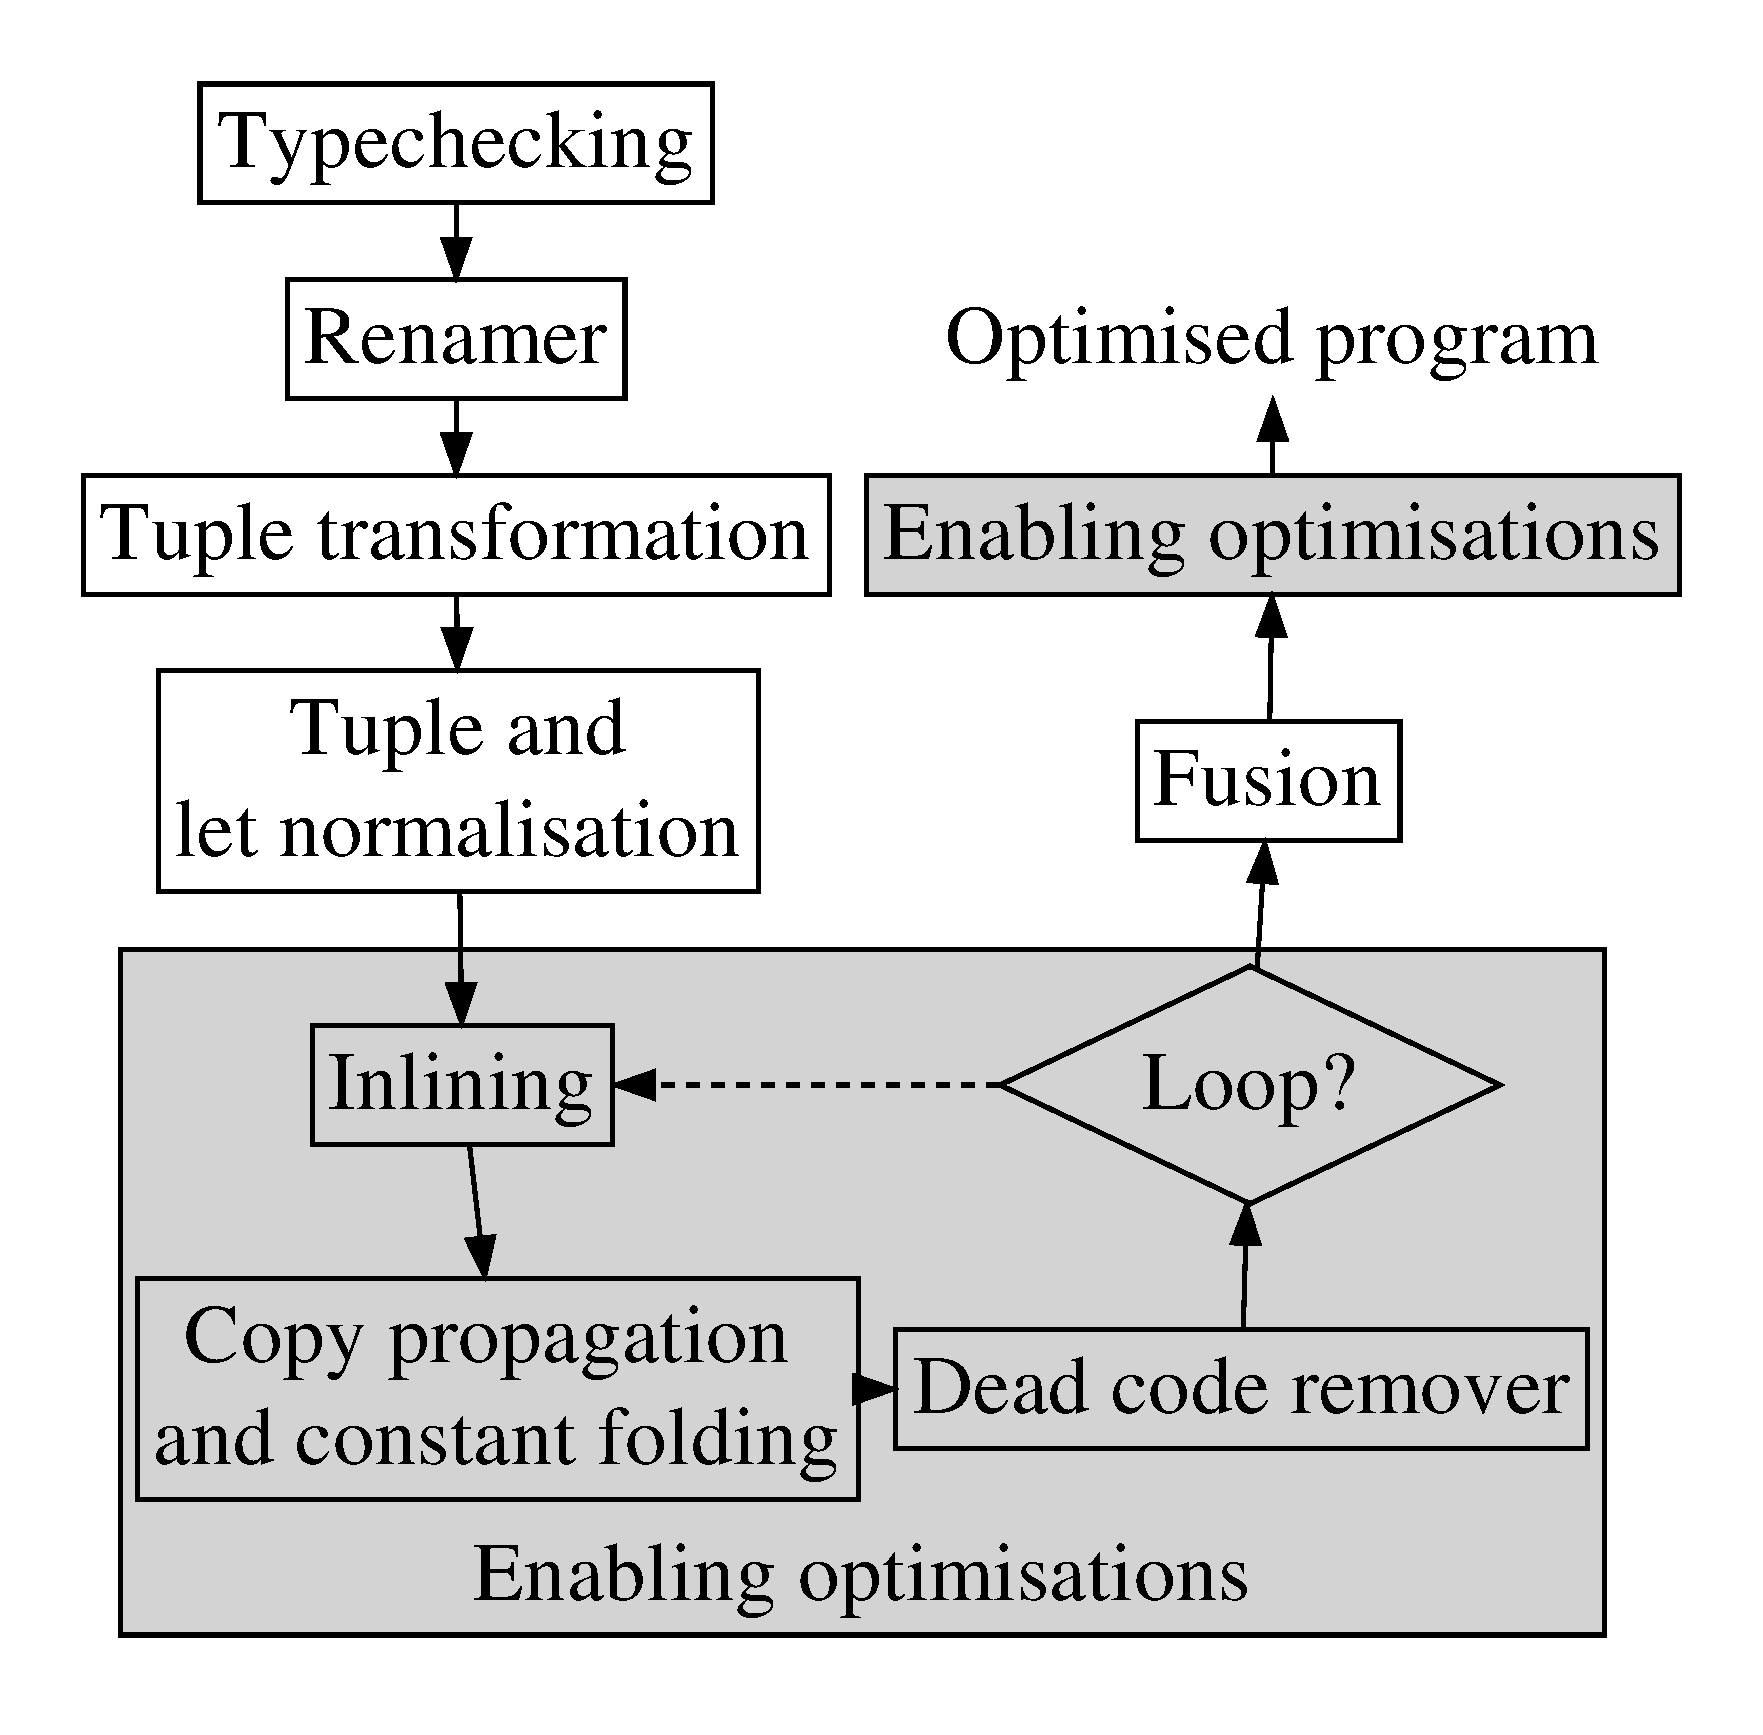
\includegraphics[width=0.7\columnwidth]{Figures/pipeline}
\end{center}
\caption{Compiler pipeline}
\label{fig:l0cpipeline}
\end{figure}

Consider the type {\tt [([int], [real])]}, which is transformed to
{\tt([[int]], [[real]])}.  These two types are not isomorphic, as the
latter has more stringent demands to the fullness of arrays.  For
example, {\tt\{(\{1\}, \{1.0\}), (\{2,3\}, \{2.0\})\}} is a value of
the former, but the first element of the corresponding transformed
tuple {\tt(\{\{1\}, \{2, 3\}\}, \{\{1.0\}, \{2.0\}\})} is not a full
array.  Hence, when determining whether a program generates full
arrays, we must look at the \textit{transformed} values - in a sense,
the fullness requirement ``transcends'' the tuples.  Also, after
tuple-transformation, {\tt zip} and {\tt unzip} disappear.

After tuple transformation, the previously described {\sc soac}s are
no longer usable, as they each accept only a single input array.
Hence, we introduce matching tuple-{\sc soac}s, which accept as input
an arbitrary number of arrays, and likewise their result is
a tuple.
%any number of input arrays, and whose return value is likewise a tuple if
%applicable.  
Their syntax is depicted in Figure~\ref{fig:tuple-soacs}, 
and their semantics is: % as below:
\begin{align*}
  \text{\tt map2} &:: (\alpha_{1}\rightarrow\ldots\rightarrow\alpha_{n})\rightarrow(\beta_{1},\ldots,\beta_{m}))\\
&\rightarrow[\alpha_{1}]\rightarrow\ldots\rightarrow[\alpha_{n}]\rightarrow([\beta_{1}],\ldots,[\beta_{m}]))
\end{align*}
\begin{align*}
  \text{\tt map2($f$,$e_{1}$,\ldots,$e_{n}$)} & \equiv \text{\tt unzip(map($f'$, zip($e_{1}$, \ldots, $e_{n}$)))}
\end{align*}
\begin{align*}
  \text{\tt reduce2} &::(\alpha_{1}\rightarrow\ldots\rightarrow\alpha_{n}\rightarrow\alpha_{1}\rightarrow\ldots\rightarrow\alpha_{n}\rightarrow(\alpha_{1},\ldots\alpha_{n}))\\
& \rightarrow(\alpha_{1},\ldots,\alpha_{n})\rightarrow[\alpha_{1}]\rightarrow\ldots\rightarrow[\alpha_{n}]\rightarrow([\alpha_{1}],\ldots,[\alpha_{n}])
\end{align*}
\begin{align*}
  \text{\tt reduce2($f$,$x$,$e_{1}$,\ldots,$e_{n}$)} &\equiv \text{\tt reduce($f'$,$x$,zip($e_{1}$,\ldots,$e_{n}$))}
\end{align*}
\noindent where $f'$ has the tuple-transformed body of $f$ and the arguments
of $f$ have been rewritten such that an original argument of tuple type is
expanded into distinct arguments.
%to accept tuple elements as distinct arguments.
The remaining {\sc soac}s are similar.    For simplicity, the
above semantics always describe the return value as a tuple.  In
practice, if this would be a one-element tuple (which is not permitted
in \LO), we use the element by itself.  The array-arguments to a
tuple-{\sc soac} must all have the same length.

\begin{figure}[bt]
\begin{tabular}{lrll}
$e$ & $::=$ & {\tt map2($l$, $e_{1}$, \ldots, $e_{n}$)} \\
    & $|$ & {\tt filter2($l$, $e_{1}$, \ldots, $e_{n}$)} \\
    & $|$ & {\tt reduce2($l$, $x_{1}$, \ldots, $x_{n}$, $e_{1}$, \ldots, $e_{n}$)} \\
    & $|$ & {\tt scan2($l$, $x_{1}$, \ldots, $x_{n}$, $e_{1}$, \ldots, $e_{n}$)} \\
    & $|$ & {\tt redomap2($l_{r}$, $l_{m}$, $x_{1}$, \ldots, $x_{n}$, $e_{1}$, \ldots, $e_{n}$)} \\
\end{tabular}
\caption{Second-order tuple-array combinators}
\label{fig:tuple-soacs}
\end{figure}

As an example, consider the following (contrived) program for
computing the dot product of an array and its inverse.

\begin{colorcode}
fun real main([real] a) =
  reduce(op +, 0.0,
         map(op *,
             map(fn (real,real) (real x) => (x,~x),
                 a)))
\end{colorcode}
Now we perform the tuple-transformation.  Note that the return value
of the first {\tt map2} is taken apart in a tuple pattern, so that it
can be passed piecewise to the next {\tt map2}.
\begin{colorcode}
fun real main([real] a) =
  let (e1, e2) =
    map2(fn (real, real) (real x) =>
         (x,~x), a) in
  let tmp_map2 =
    map2(fn real (real x, real y) => x * y,
         e1, e2) in
  let tmp_red2 =
    reduce2(fn real (real x, real y) =>
            x + y, 0.0, tmp_map2) in
  tmp_red2
\end{colorcode}

%%%%%%%%%%%%%%%%%%%%%%%%%%%%%%%%%%%%%%%%%%%%%%%%%%%%%%%%%%%%%%%%%%%%
%%%%%%%%%%%%%%%%%%%%%%%%%%%%%%%%%%%%%%%%%%%%%%%%%%%%%%%%%%%%%%%%%%%%
%%%%%%%%%%%%%%%%%%%%%%%%%%%%%%%%%%%%%%%%%%%%%%%%%%%%%%%%%%%%%%%%%%%%
\section{Fusion: A Structural-Analysis Transformation}

The fusion transformation, presented in this section, assumes a {\em
  normalized} program, i.e., by running the transformations introduced
in Section~\ref{sec:Prelim} to obtain the properties listed in
Section~\ref{sec:compiler-pipeline}

\begin{figure}[bt]
%\hrule ~
\vbox{
\begin{center}
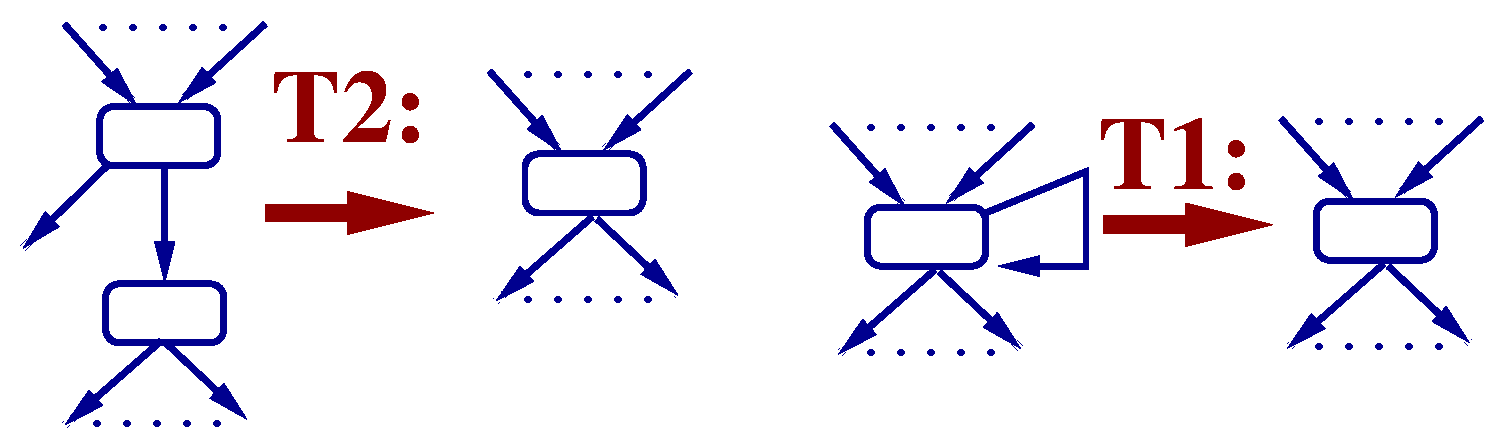
\includegraphics[height=17ex]{Figures/CFG_T12}
\end{center}
}
\caption{T$_1$-T$_2$ Transformation For Testing CFG Reducibility}
\label{fig:T1T2}
\end{figure}

Structural analysis is rooted in the T$_1$-T$_2$ transformation~\cite{T12}
depicted in Figure~\ref{fig:T1T2}.
If repeated application of T$_1$ and T$_2$ to a control-flow graph ({\sc cfg}) 
results in one point, then the {\sc cfg} is said to be reducible, i.e.,
the code can be re-written using only regular (while) {\tt loop}s, 
{\tt if} and {\tt goto}-free statements (with function calls).

Data-flow optimizations on reducible {\sc cfg}s can be modeled via equations 
that are applied at each T$_1$/T$_2$ reduction, and consequently only one
{\sc cfg} pass is required instead of a fixed-point iteration.
%
In practice, if the {\sc cfg} is known to be reducible, then 
analysis can be conveniently performed source to source: 
%In practice, a reducible {\sc cfg} enables convenient source-to-source transformations: 
data-flow equations are associated directly with the
language constructs and dictate, for example, how the analysis result is
initialized at statement level, composed between consecutive statements,
merged across branches, aggregated across loops, and translated across 
call sites.  (An example of such non-trivial 
analysis is the summarization~\cite{HybAn} of array references into 
read-write, write-first and read-only set expressions, used in the context 
of array-{\sc ssa} and autoparallelization.)
 
Since \LO{} guarantees a reducible {\sc cfg}, %at function level,
fusion is implemented as an intra-procedural\footnote{
The current version of the \LO{} compiler 
relies on aggressive inlining and does not support
(yet) inter-procedural analysis.
}
source-to-source transformation: a bottom-up traversal of the 
abstract-syntax tree (\textsc{AbSyn}) builds the ``fusion kernels'' 
and a second pass substitutes them in the \textsc{AbSyn} and 
cleans up the code.    Such an approach is not uncommon. 

{\em What is less common} is that the data-flow equations 
themselves model $T_2$-like reducibility of the data-dependency graph.
The remaining of this section is organized as follows:
Section~\ref{sec:Intuition} gives the gist of the technique,
and shows several don't-fuse cases, which would
either lead to illegal programs or to duplicated computation.
%
Section~\ref{sec:FusingOnce} introduces the data structure
that stores the result of the first pass, and discusses the rules 
for processing one {\sc soac} node, including the compositional
algebra under which {\sc soac}s are fused. 
Finally, Section~\ref{sec:bwdPass} describes the data-flow rules of
the first pass for the rest of \textsc{AbSyn} nodes, and briefly 
discusses the second pass of the analysis.
%and remarks on the asymptotical 
%complexity of the transformation.

%%%%%%%%%%%%%%%%%%%%%%%%%%%%%%%%%%%%%%%%%%%%%%%%%%%%%%%%%%%%%%%%%%%%
\subsection{Motivation and Intuitive Solution}
\label{sec:Intuition}

\begin{figure}[bt]
%\hrule ~
\vbox{
\begin{minipage}{0.46\columnwidth}
\begin{center}
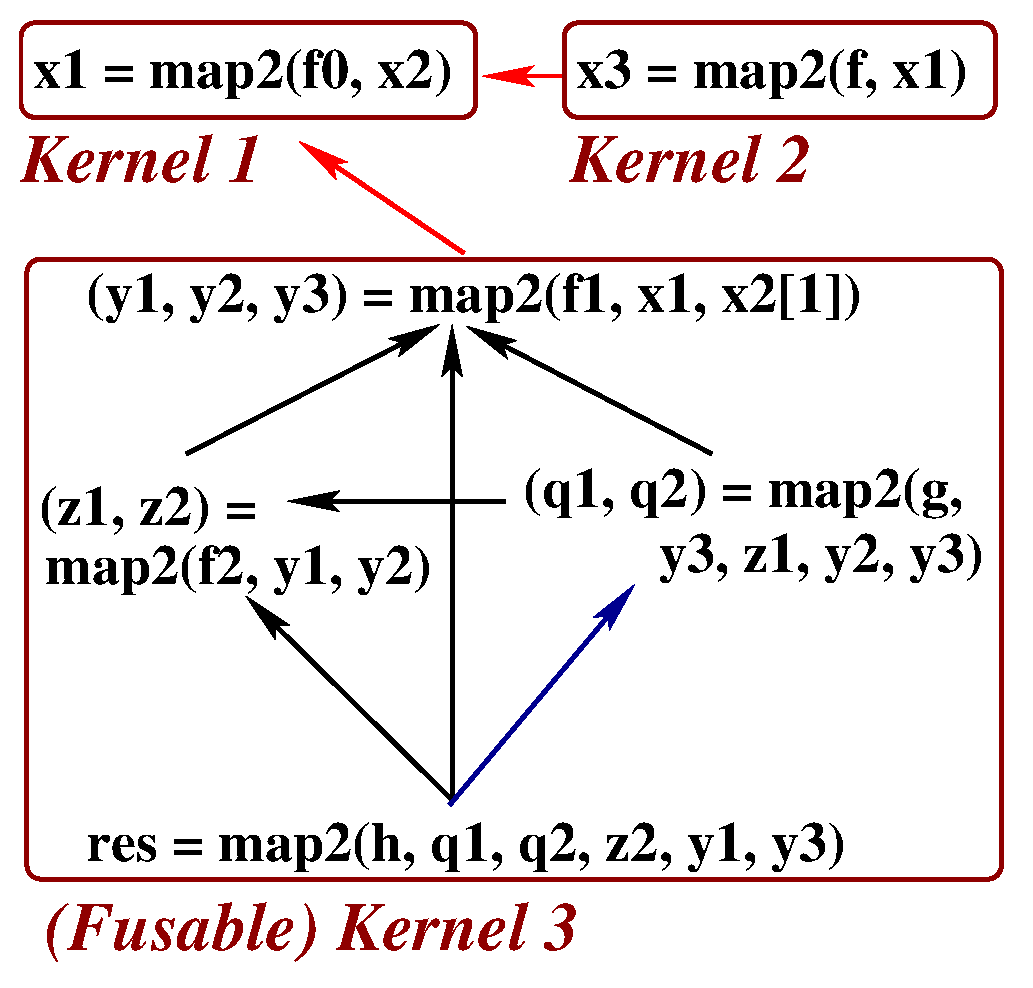
\includegraphics[height=30ex]{Figures/T1T2} \\\vspace{2ex}
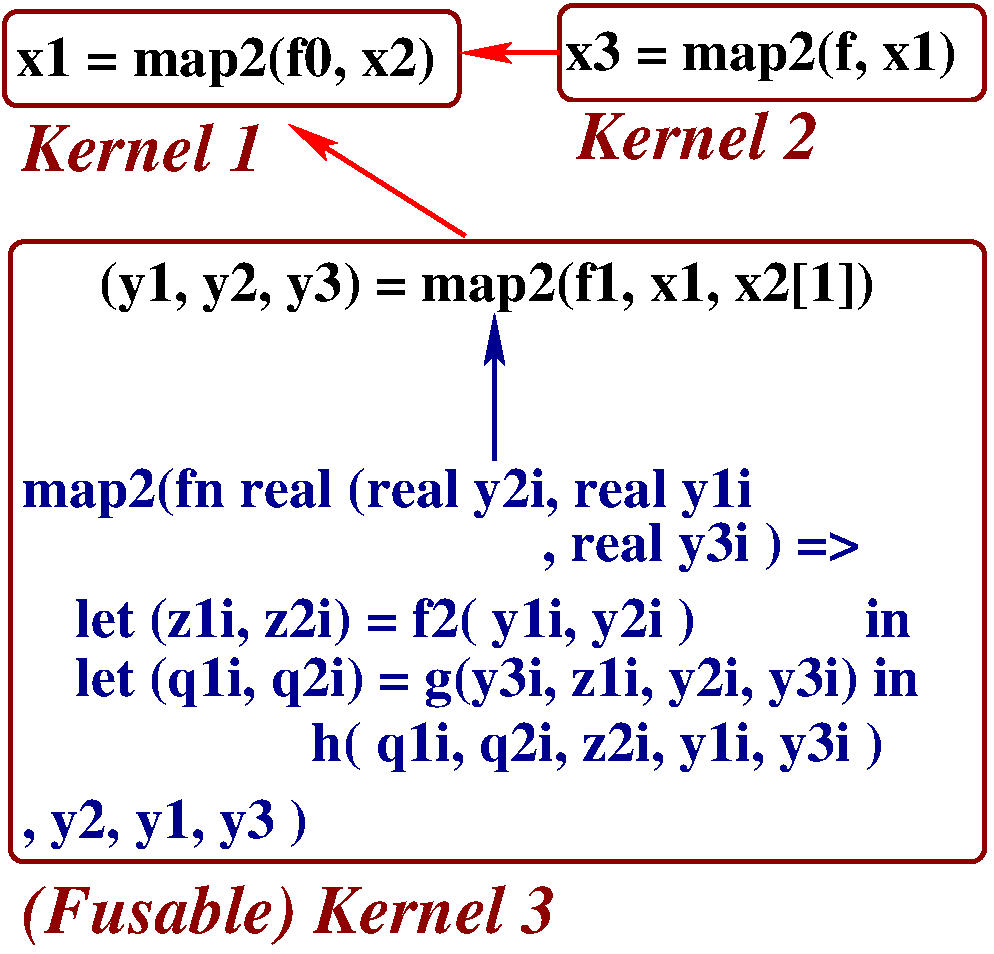
\includegraphics[height=30ex]{Figures/T1T2Fuse2}
\end{center}
\end{minipage}
\hfill
\begin{minipage}{0.46\columnwidth}
\begin{center}
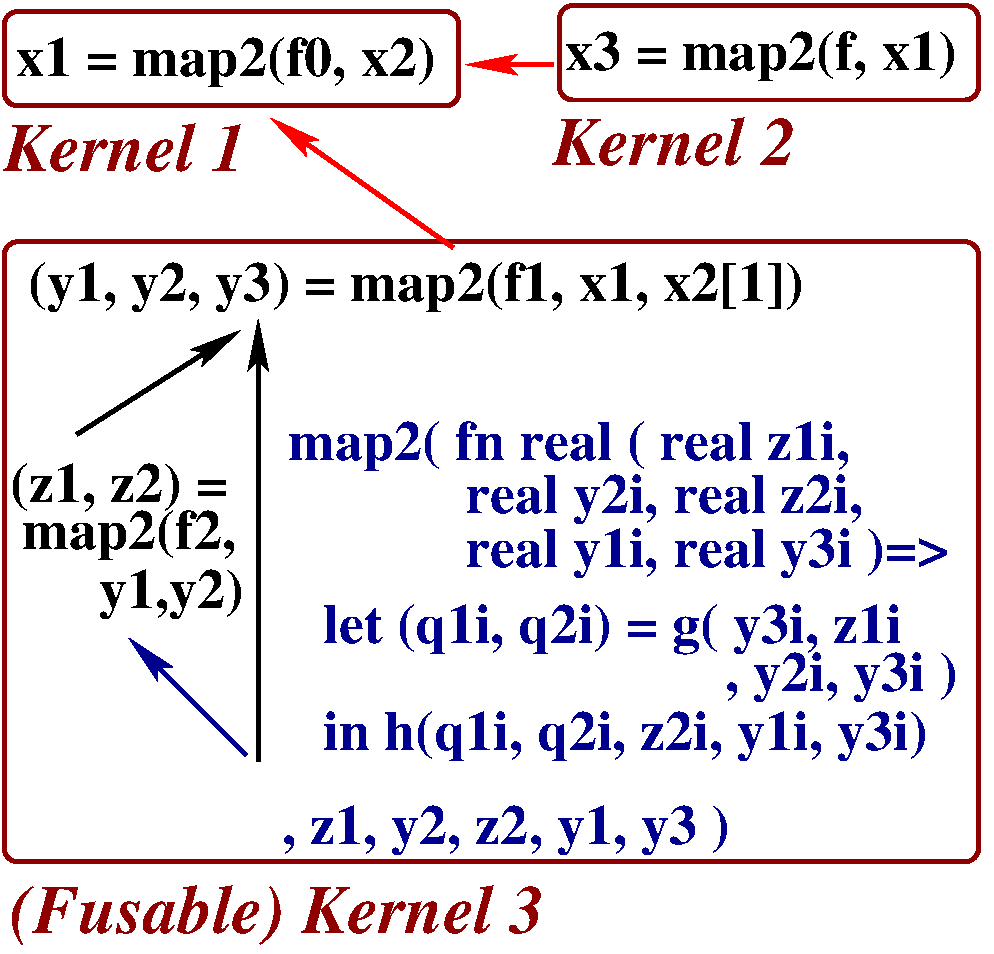
\includegraphics[height=30ex]{Figures/T1T2Fuse1} \\\vspace{2ex}
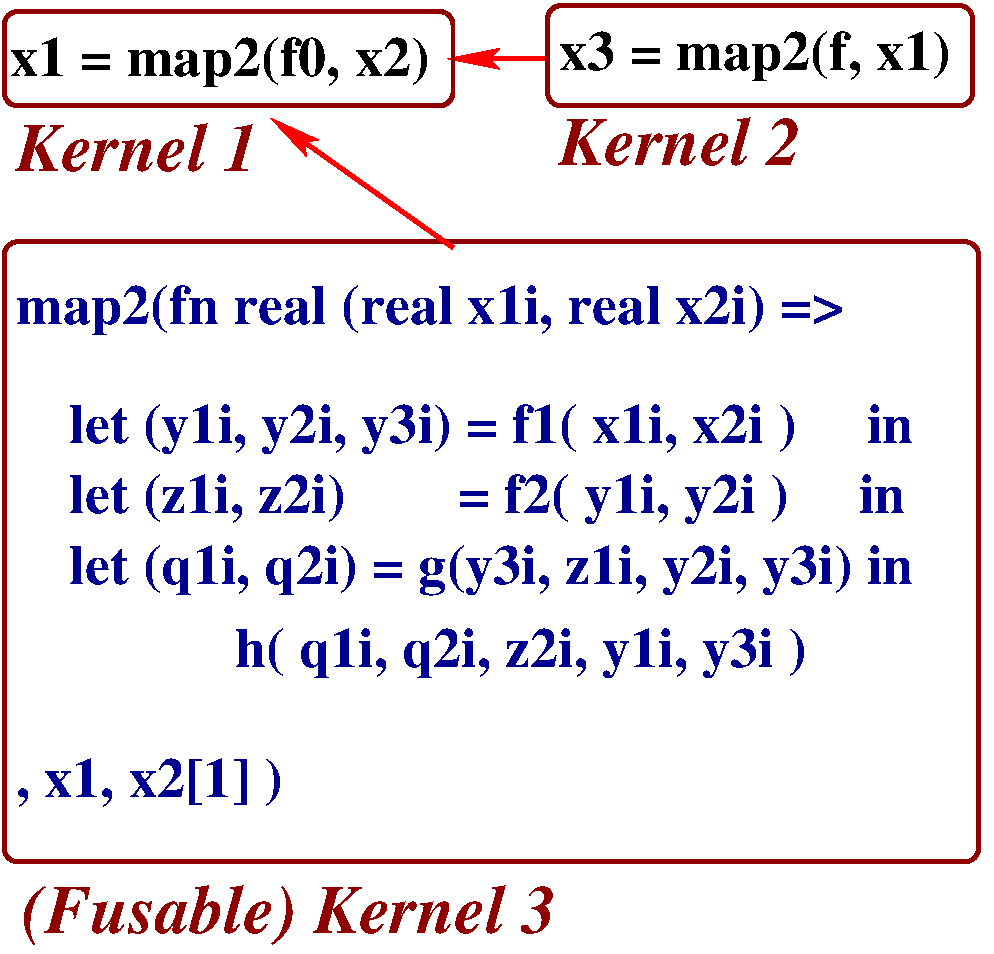
\includegraphics[height=30ex]{Figures/T1T2Fuse3}
\end{center}
\end{minipage}
}
\caption{Fusion By T2 Transformation on the Dependency Graph}
\label{fig:T1T2}
\end{figure}

Figure~\ref{fig:T1T2} depicts the intuitive idea on which
our fusion analysis is based.   The top-left figure shows
the dependency graph of a simple program, where an 
arrow points from the consumer to the producer. 
%
For simplicity, array variables are used only as input or 
output to {\sc soac} calls and the control flow is trivial,
i.e., a basic block. 

The main point is that all {\sc soac}s that appear inside the box
labeled \emp{\em Kernel 3} can be fused without duplicating any
computation, even if several of the to-be-fused 
arrays are used in different {\sc soac}s, e.g., {\tt y1} is used to
compute both {\tt (z1,z2)} and {\tt res}\footnote{
Note also that (i) not all input arrays of a {\sc soac} need to be produced
by the same {\sc soac}, e.g., the {\tt q}s requires both {\tt y}s and 
{\tt z}s arrays, and (ii) some input might be produced other than 
by a {\sc soac}, e.g, \emp{\em Kernel 3} is still fusable even if 
we add an arbitrary array as an extra parameter to the root {\tt res=map2(..)}. 
}. 
This is accomplished by means of {\em {\tt T$_2$} reduction on the dependency graph}:

The rightmost child, i.e., {\tt map2(g,..)}, of the root {\sc soac} 
has only one incoming edge, 
hence it can be fused (reduced). This is achieved  (i) by replacing in
the root {\sc soac} the child's output with the child's input arrays, 
(ii) by inserting in the root's lambda a call to the child's lambda,
which computes the per-element output of the child, %% intermediate, 
and, finally, (iii) by removing the duplicate input arrays of the resulted {\sc soac}.
The latter introduces copy statements for all but one 
of the (former) arguments of the lambda corresponding to the same duplicated
array (and removes those former arguments).

%replacing in the result's lambda
%the definition of all but one of the lambda's arguments corresponding to 
%the same input array, with copy statements in the lambda's body.  

The top-right part of Figure~\ref{fig:T1T2} shows in blue the (optimized) 
result of the first fusion, where the copy statements have been eliminated 
by copy propagation.   In the new graph, the leftmost child of the root, 
i.e., the one computing {\tt (z1,z2)}, has only one incoming edge 
and can be fused.  The resulted graph, shown in the bottom-right Figure
can be fused again resulting in the bottom-left graph of Figure~\ref{fig:T1T2}.
At this point no further {\tt T}$_2$ reduction is possible because
the {\sc soac} computing {\tt x1} has two incoming edges. 
%
{\em When no {\tt T}$_2$ reduction is possible a new kernel is started}, 
e.g., \emp{\em Kernel 1}.


\begin{figure}[bt]
%\hrule ~
\vbox{
\begin{minipage}{0.48\columnwidth}
\begin{colorcode}
// \emp{Case 1:} don't fuse if it
//moves an array use across 
//its in-place update point
let \emphh{x}   = map2(f, \emp{a}) in
let \emp{a}[1]= 3.33       in
let y   = map2(g, \emp{x}) in ..

// \emp{Case 3:} don't fuse from 
//outside in a loop (or \mymath{\lambda})
let \emphh{x} = map2(f, a)   in
\emp{loop}(arr) = for i < N do
  map2(op +, arr, \emp{x})

// \emp{Case 5:} don't fuse if \emp{x}
//used outside SOAC inputs
let \emphh{x} = map2(f, a) in
let y = map2(g, \emphh{x})   in
    \emp{x}[i] + y[i]
\end{colorcode}
\end{minipage}
\hfill
\begin{minipage}{0.48\columnwidth}
\begin{colorcode}
// \emp{Case 2:} not all SOAC
//combinations are fusable
let \emp{x} = filter2(c\mymath{\myindx{1}}, a) in
let \emp{y} = filter2(c\mymath{\myindx{1}}, b) in
let z = map2   (f,\emp{x,y}) in..

// \emp{Case 4:} don't fuse in 2
//kernels sharing a CF path
let \emphh{x} = map2(f, arr)  in
let y = if c then map2(g\mymath{\myindx{1}},\emphh{x}) 
             else map2(g\mymath{\myindx{2}},\emphh{x})
in let z = map2(h, \emp{x}) in ..

// \emp{Case 6:} x \& y used exactly
//once but still don't fuse
let (\emphh{x},\emphh{y}) = map2(f, a)   in
let u = reduce2(op +,0,\emp{x})in
let v = reduce2(op *,1,\emp{y})..
\end{colorcode}
\end{minipage}
%\begin{center}
%\includegraphics[height=12ex]{figures/MemCoalesce}
%\end{center}
} 
%\vspace{-1ex}
\caption{Don't Fuse Cases: Illegal or Duplicates Computation}
\label{fig:dontFuse}
\end{figure}

Having presented the intuitive idea, we look next at six cases,
depicted in Figure~\ref{fig:dontFuse}, where fusion is disallowed because
it would result either in incorrect programs or in duplicated computation:
\begin{itemize}
    \item [1.] A {\sc soac} {\tt s} cannot be fused across the 
                ``in-place update'' of an array {\tt a} if {\tt s} uses any 
                variable in the alias set of {\tt a}.  Otherwise, fusion would
                violate \LO's semantics because an alias of {\tt a} is used on 
                an execution path following {\tt a}'s in-place update.
    \item [2.] Not all combinations of {\sc soac}s are fusable. For example,
                a {\tt map} whose input arrays are produced by two {\tt filter} 
                operations can be fused as a loop, but this is not useful
                due to the sequential nature of the resulted loop, i.e., it 
                uses two induction variables without closed-form solutions.
    \item [3.] Fusing across a loop (or a {\sc soac}'s lambda) would 
                duplicate computation and potentially change the  
                time complexity of the program, because the loop-invariant
                computation of the producer would be redundantly executed 
                loop-count times. 
    \item [4.] If a {\sc soac}-produced array {\tt x} is consumed by two other
                {\sc soac}s at two program points located on the same execution 
                path $p$ then the fused program would compute {\tt x} twice on $p$. 
                However, if the two program points are located on disjoint execution 
                paths then fusion is allowed. For example, if the {\tt map2} computing 
                {\tt z} is removed, then fusing the {\tt x} producer in the 
                {\tt then} and {\tt else} branches does not duplicate computation.
    \item [5.] If a {\sc soac}-produced array {\tt x} is used other than input to   
                another {\sc soac} then fusing {\tt x} is disallowed in our 
                implementation.   A future extension might handle the ``negligible-overhead'' 
                cases, e.g., substituting {\tt x[i]} with {\tt f(arr[i])} 
                would allow the fusion of {\tt x} at the cost of computing {\tt f(arr[i])} (twice).
    \item [6.] Finally, fusing two arrays produced by the same {\sc soac} each in another
                {\sc soac} still duplicates computation. This case can sometimes
                be optimized by ``horizontally'' merging the {\sc soac} consumer,
                e.g., the two {\tt reduce2}s are merged in {\tt reduce2(g,0,1, x,y)},
                where {\tt g(e$_1$,e$_2$,x$_i$,y$_i$)~$\equiv$~(e$_1$+x$_i$, e$_2$*y$_i$)}.
\end{itemize}

We conclude this section with two remarks: {\em First}, the data-dependency  % in practice
graph ({\sc ddg}) does not have to be built since a bottom-up traversal of the program, 
i.e., backwards analysis, is guaranteed to encounter the statements\footnote{
Fusion assumes a normalized program, i.e., seen as a set of functions 
whose bodies are composed from blocks of let-statements, {\tt if}s and {\tt loop}s.
} in an order that satisfies the {\sc ddg}.
{\em Second}, the intuition is not complete, as it does not solve the 
issues described in the ``don't fuse'' cases, e.g., violation of the ``in-place update'' 
semantics, handling fusion across loops and branches, etc. 
%
The next two sections present in detail the backward-analysis pass.
  

%%%%%%%%%%%%%%%%%%%%%%%%%%%%%%%%%%%%%%%%%%%%%%%%%%%%%%%%%%%%%%%%%%%%
\subsection{Fusing One SOAC}
\label{sec:FusingOnce}

\begin{figure}[bt]
%\hrule ~
\vbox{
\begin{minipage}{0.48\columnwidth}
\begin{colorcode}
import qualified Data.Map 
                 as M
import qualified Data.Set 
                 as S
data \emp{FusedKer} = \emp{FusedKer} \{ 
 \emphh{soacStmt} :: ([Name], Exp)
--^the fused SOAC stmt,eg,
--(z,w)=map2( f(a,b), x,y )

,\emphh{inp}     :: S.Set Name
--^ the input arrays used   
--in SOAC stmt,i.e.,\{x,y\}.

,\emphh{inplace} :: S.Set Name
--^Aliasing set of vars
--used in in-place updates
--that reach this kernel.

,\emphh{fused_vars} :: [Name]
--^not null iff at least a 
--fusion has been performed
\}
\end{colorcode}
\end{minipage}
\hfill
\begin{minipage}{0.48\columnwidth}
\begin{colorcode}
data \emp{FusionRes} = \emp{FusionRes}\{
 \emphh{outArr} :: M.Map Name Name
--^maps an array to the name
--of the kernel producing it 

,\emphh{inpArr} :: M.Map  Name 
                (S.Set Name)
--^maps an array to the 
--names of kernels using it  

,\emphh{unfusable} :: S.Set Name
--^Unfusable arrays. Used:
--1.otherwise than input to 
--  SOAC kernels (including
--  lambda bodies), or 
--2.as input to two kernels 
--  not located on disjoint 
--  control-flow (branches)

,\emphh{kers} ::M.Map Name FusedKer
--^maps kernel name to data
\}
\end{colorcode}
\end{minipage}
} 
\caption{Data Structures for Fusion Metadata.}
\label{fig:fusionDS}
\end{figure}

%\enlargethispage{\baselineskip}

Figure~\ref{fig:fusionDS} shows the representation of the data-flow result
computed during the bottom-up analysis pass, i.e., synthesized attribute.  
A fused kernel, \emp{\tt FusedKer}, consists of:
\begin{itemize}
    \item the {\sc soac} statement, {\tt soacStmt}, which pairs up
            the output arrays produced by the fused {\sc soac} 
            with the {\sc soac}'s \textsc{AbSyn} expression,
            %({\tt Ident} records a variable's name, type and position), 
    \item the set of input arrays, {\tt inp}, of the fused {\sc soac},
    \item a set of variable names, {\tt inplace}, which is
            the union of the alias sets of all arrays that may have 
            been ``consumed\footnote{
                An array is consumed either (i) when it is the 
                source of an in-place update or (ii) when it is passed 
                to a function call as a parameter of unique type. 
            }''
            on any execution path between the currently-analyzed program 
            point to the one where the fused {\sc soac} was called; e.g.,
            in \emp{Case 1} of Figure~\ref{fig:dontFuse}, {\tt a}
            belongs to the {\tt inplace} set of the kernel associated
            with output {\tt y}, when analysis reaches 
            the definition of {\tt x},
    \item a set of array variables, {\tt fused\_vars}, that have been 
            fused in the construction of the current kernel;
            if {\tt fused\_vars $=\emptyset$} then no fusion has
            yet taken place, and {\tt soacStmt} is in the program.       
\end{itemize}

The analysis result is implemented by the \emp{\tt FusionRes} structure: 
\begin{itemize}
    \item {\tt outArr} maps an array name to the kernel (name) producing it, 
    \item {\tt inpArr} maps an array name {\tt x} to the set of kernels (names) 
            whose corresponding {\sc soac}s receive {\tt x} as an input array,
    \item a set of array names that the analysis up to the current 
            program point have discovered to be {\tt unfusable}, because
            of one of the \emp{cases 3 to 6} in Figure~\ref{fig:dontFuse},
            e.g., arrays used other than {\sc soac} input or
            in two different kernels that share an execution path, etc., and
    \item {\tt kers} maps a kernel name to its associated \emp{\tt FusedKer} data.
\end{itemize}

\begin{figure}[bt]
%\hrule ~
\vbox{
\begin{colorcode}
data \emphh{FusionEnv} = FusionEnv \{
    \emphh{soacsEnv} :: M.Map Name ([Name], Exp)
    --^ maps array names to their producing SOAC stmt
  , \emphh{varsEnv}  :: S.Set Name 
    --^ set of in-scope variables at current prog point
\}
newtype \emp{FusionM} a = FusionM (StateT NameSrc 
               (ReaderT FusionEnv (Either FusionErr)) a)
  deriving ( MonadState  NameSrc, MonadReader \emphh{FusionEnv},
             Monad, Applicative, Functor )

\emp{tryFuseSOAC}:: S.Set Name     ->         FusionRes -> 
             -- vars \mymath{\in} SOAC's lamba,   current result  
              ([Name], Exp) -> \emp{FusionM} FusionRes
             -- SOAC stmt,      result after fusion
\emp{tryFuseSOAC} lam_vars res (out_nms, soac) = do   
  inp_ids <- getInpArrsSOAC soac
  -- e.g., [x,y] \mymath{\Leftarrow} map2(f, x, y)  
  inp_nms <- \emphh{expandSOACsInpArr} \$ inp_ids
  -- e.g., [x,y] \mymath{\Leftarrow} map2(g, x) {\em if} let (x,y) = map2(f,a) 
    
  -- \emp{Conditions for fusion:}
  --(1) \emphh{none of out_nms belongs to the unfusable set}
  let cond1=L.all(\mymath{\backslash}x->not\$S.member x\$unfusable res) out_nms 

  --(2) \emphh{\mymath{\exists} some kernels that use some of out_nms as inputs} 
  let to_fuse_knms = getKersWithInpArrs res out_nms
  to_fuse_kers <- mapM (\mymath{\backslash}x-> case M.lookup x (kers res) of
                              Nothing -> fusionErrorM ...
                              Just ker-> return ker
                       ) to_fuse_knms
  --(3) \emphh{all kernels have to be compatible for fusion}, 
  --    \emphh{e.g., map2 o filter2 not supported}
  let all_compat = L.all (isCompatibleKer out_nms soac) 
                         to_fuse_kers
  --(4) \emphh{fusion cannot move a use of an input array}
  --    \emphh{past its in-place update}
  let all_used=foldl (\mymath{\backslash}y x->S.insert x y) lam_vars inp_ids
  let ok_inplace = L.all S.null \$ 
    map (S.intersection all_used . inplace) to_fuse_kers 

  let all4_ok = cond1 && not \$ null to_fuse_kers && 
                all_compat && ok_inplace
  -- \emp{Update Unfusable Set} \emphh{with the input-array names that}
  -- \emphh{appear as input arrays in kernels \mymath{\notin} to_fuse_kers},
  -- \emphh{since those are input to at least 2 distinct kernels.}
  let mod_kers=if is_fusable then to_fuse_knms else []
  let in2_kers=filter (inpArrInRes res mod_kers) inp_nms
  let unfus'=S.union (unfusable res) (S.fromList in2_kers)
  let res' = res \{ unfusable = unfus' \}

  if not all4_ok then mkNewKernel res' (out_nms,soac)
             -- adds a fresh kernel to the result, and    
             -- updates the outArr and inpArr fields
  else do fused_kers <- mapM (fuseSOACInKer out_nms soac) 
                             to_fuse_kers
          -- fuses current soac with all to_fuse_kers
          updateFusionRes res' fused_kers to_fuse_knms
          -- updates out/inpArr \& kers fields of result
\end{colorcode}
} \vspace{-2ex}
\caption{ Pseudo-code for Conservatively Fusing one {\sc soac} }
\label{fig:FuseOnce}
\end{figure}


Figure~\ref{fig:FuseOnce} shows % the monadic types used in our implementation and 
the Haskell pseudo-code that implements the most important 
analysis step: the one that gives the data-flow rules for processing 
a {\sc soac} statement, \emp{\tt tryFuseSOAC}. 
%
The analysis uses an environment, \emphh{\tt FusionEnv}, that records the set 
of array variables visible at the current program point, {\tt varsEnv}, and a 
map binding array names to the {\sc soac} statement producing it, {\tt soacsEnv}. 
The environment is computed during the top-down \textsc{AbSyn} traversal, 
i.e., an inherited attribute.
%
The computation takes place in the \emp{\tt FusionM} monad that is a
composition of (i) the {\tt Reader} monad, for maintaining the environment,
(ii) the {\tt State} monad, for fresh-names generation, and (iii) the 
{\tt Either} monad, for error handling.

Function \emp{\tt tryFuseSOAC} receives as arguments (i) the set of variables
that are visible in the current scope and are used in the current-{\sc soac}'s
lambda, {\tt lam\_vars}, (ii) the current data-flow result, {\tt res}, and
(iii) the output arrays and the expression of the to-be-processed 
{\sc soac} statement, {\tt (out\_nms,soac)}.  

There are four conditions, {\tt all4\_ok}, that have to be met for the 
current {\sc soac}, denoted {\sc s}$_c$, to be fused with at least one kernel: %existent
\begin{itemize}
    \item [1.] None of {\tt soac}'s output-array names, {\tt out\_nms}, 
                belong to the result's {\tt unfusable} set.
    \item [2.] There exists some kernels, {\tt to\_fuse\_kers}, found by look-ups
                in the result's {\tt inpArr}, whose input arrays belong to {\tt out\_nms}.
                If the previous condition is met then it is guaranteed (see Section~\ref{sec:bwdPass}) 
                that all {\tt to\_fuse\_kers} are located on disjoint execution paths,
                and that none of them are in a loop or lambda 
                that does not contain {\sc s}$_c$, 
                i.e., \emp{Cases 2 to 6} of Figure~\ref{fig:dontFuse} do not happen.
    \item [3.] All kernels in {\tt to\_fuse\_kers} are compatible with 
                    {\sc s}$_c$ under the algebra depicted 
                    in Figure~\ref{fig:CompatFuse} and reviewed later. 
               Otherwise, if only some kernels are compatible, then computation
                will be duplicated since {\sc s}$_c$ cannot be removed
                from the program.
    \item [4.] None of {\sc s}$_c$'s variables, including the
                ones used in its lambda and as input arrays, belong to the 
                {\tt inplace} set of any kernels in {\tt to\_fuse\_kers}.
                Otherwise, \emp{Case 1} of Figure~\ref{fig:dontFuse} may apply.
\end{itemize}

The next step is to update the {\tt unfusable} set of the data-flow result.
At this stage the variables used in the current {\sc soac} ({\sc s}$_c$) lambda
have been already made unfusable. It remains to check whether any input
array\footnote{
A normalized program guarantees that the input arrays of a {\sc soac}
are variables rather than arbitrary expressions, hence we need not scan them.
} of {\sc s}$_c$, i.e., {\tt inp\_nms}, is also used in an 
existing kernel. If so, then it is used in at least two kernels that may
share an execution path, and hence it is unfusable. There are two things 
to be noted here:
{\em First}, if an array in the input set of {\sc s}$_c$
was produced by another {\sc soac}, {\sc s}$_2$, then {\tt inp\_nms} is
extended with all output arrays of {\sc s}$_2$; otherwise \emp{Case 6} 
of Figure~\ref{fig:dontFuse} may apply. This is achieved by
{\tt expandSOACsInpArr} via looks-ups in \emphh{soacsEnv}. 

{\em Second}, an input array, {\tt a}, does {\em not} become unfusable if
{\sc s}$_c$ can be fused {\em and} {\tt a} is used only as input 
to the kernels with which {\sc s}$_c$ will be fused. In this case {\tt a}
would still be used only in kernels located on disjoint execution paths
(This is implemented by filtering modulo kernels 
{\tt mod\_kers} in the  definition of {\tt in2\_kers}.)


\begin{figure}[bt]
%\hrule ~
\vbox{
\begin{minipage}{0.48\columnwidth}
\begin{colorcode}
// \emp{replicate can be fused}
//\emp{without restrictions}
let x = replicate(N,a)in 
let y = map2(f, x, b) in
let z = map2(g, x, c) in 
let x[i] = ...
    \emphh{\mymath{\equiv}}
let x = replicate(N, a) in 
let y = map2( fn \mymath{\beta\myindx{1}} (\mymath{\alpha\myindx{1}} b\mymath{\myindx{i}}) 
              => f(a,b\mymath{\myindx{i}}), b)
let z = map2( fn \mymath{\beta\myindx{2}} (\mymath{\alpha\myindx{2}} c\mymath{\myindx{i}}) 
              => g(a,c\mymath{\myindx{i}}), c)
in let x[i] = ...   


//\emp{map2 o map2 \mymath{\Rightarrow} map2}  
let (x1, x2) = map2(f, a1)
in  map2(g, x1, y)   
    \emphh{\mymath{\equiv}}
map2(fn \mymath{\beta} (\mymath{\alpha\myindx{1}} a1\mymath{\myindx{i}}, \mymath{\alpha\myindx{2}} y\mymath{\myindx{i}})
  =>let (x1\mymath{\myindx{i}}, x2\mymath{\myindx{i}}) = f(a1\mymath{\myindx{i}})
    in  g(x1\mymath{\myindx{i}}, y\mymath{\myindx{i}})
, a1, y )


//\emp{reduce2 o map2\mymath{\Rightarrow}redomap2}
let (x1, x2) = map2(f, a1)
in  reduce2(\mymath{\oplus},e\mymath{\myindx{1}},e\mymath{\myindx{2}}, x1,y)   
    \emphh{\mymath{\equiv}}
redomap2(\mymath{\oplus}
, fn (\mymath{\beta\myindx{1}},\mymath{\beta\myindx{2}}) ( \mymath{\beta\myindx{1}} e\mymath{\myindx{1}}, \mymath{\beta\myindx{2}} e\mymath{\myindx{2}}
             , \mymath{\alpha\myindx{1}} a1\mymath{\myindx{i}},\mymath{\alpha\myindx{2}} y\mymath{\myindx{i}})
   => let (x1\mymath{\myindx{i}}, x2\mymath{\myindx{i}}) = f(a1\mymath{\myindx{i}})
      in  \mymath{\oplus}(e\mymath{\myindx{1}},e\mymath{\myindx{2}},x1\mymath{\myindx{i}},y\mymath{\myindx{i}})
, (e\mymath{\myindx{1}}, e\mymath{\myindx{2}}), a1, y )


//\emp{redomap2 o map2\mymath{\Rightarrow}redomap2}
let (x1, x2) = map2(f, a1)
in  redomap2(\mymath{\oplus}, g, e, x1, y)
    \emphh{\mymath{\equiv}}
redomap2(\mymath{\oplus}
, fn \mymath{\beta} (\mymath{\beta} e, \mymath{\alpha\myindx{1}} a1\mymath{\myindx{i}}, \mymath{\alpha\myindx{2}} y\mymath{\myindx{i}})
   => let (x1\mymath{\myindx{i}}, x2\mymath{\myindx{i}}) = f(a1\mymath{\myindx{i}})
      in  g(e, x1\mymath{\myindx{i}}, y\mymath{\myindx{i}})
, e, a1, y )
\end{colorcode}
\end{minipage}
\hfill
\begin{minipage}{0.48\columnwidth}
\begin{colorcode}
//\emp{filter2 o filter2\mymath{\Rightarrow}filter2}
//\emp{{\em{}IFF} consumer's input set}
//\emp{  \mymath{\subseteq} producer's output set}
let (x1,x2)=filter2(c\mymath{\myindx{1}},a1,a2)
in  let y = filter2(c\mymath{\myindx{2}}, x1) ..
    \emphh{\mymath{\equiv}}
let (y, dead) = filter2(
  fn bool (\mymath{\alpha\myindx{1}} a1\mymath{\myindx{i}},\mymath{\alpha\myindx{2}} a2\mymath{\myindx{i}})=> 
      if   c\mymath{\myindx{1}}(a1\mymath{\myindx{i}}, a2\mymath{\myindx{i}}) 
      then c\mymath{\myindx{2}}(a1\mymath{\myindx{i}}) 
      else false 
, a1, a2 ) ..

//\emp{reduce2 o filter2\mymath{\Rightarrow}redomap2}
//\emp{{\em{}IFF} consumer's input list}
//\emp{  \mymath{\equiv} producer's output list}
let x = filter2(c, a)
in  reduce2(\mymath{\oplus}, e, x)
    \emphh{\mymath{\equiv}}
reduce2(fn \mymath{\beta} (\mymath{\beta} e, \mymath{\beta} a\mymath{\myindx{i}}) =>
  if c(a\mymath{\myindx{i}}) then \mymath{\oplus}(e,a\mymath{\myindx{i}}) else e
, e, a )

//\emp{reduce2 o filter2\mymath{\Rightarrow}redomap2}
//\emp{{\em{}IFF} consumer's input set}
//\emp{  \mymath{\subseteq} producer's output set}
let (x1,x2)=filter2(c, a1, a2)
in  reduce2(\mymath{\oplus}, e, x1)
    \emphh{\mymath{\equiv}}
redomap2(\mymath{\oplus}
, fn \mymath{\beta} (\mymath{\beta} e, \mymath{\alpha\myindx{1}} a1\mymath{\myindx{i}}, \mymath{\alpha\myindx{2}} a2\mymath{\myindx{i}})
   => if c(a1\mymath{\myindx{i}}, a2\mymath{\myindx{i}})
      then \mymath{\oplus}(e, a1\mymath{\myindx{i}}) else e
, e, a1, a2 )

//\emp{redomap2 o filter2\mymath{\Rightarrow}redomap2}
//\emp{{\em{}IFF} consumer's input set}
//\emp{  \mymath{\subseteq} producer's output set}
let (x1,x2)=filter2(c, a1, a2)
in  redomap2(\mymath{\oplus}, g, e, x1)
    \emphh{\mymath{\equiv}}
redomap2(\mymath{\oplus}
, fn \mymath{\beta} (\mymath{\beta} e, \mymath{\alpha\myindx{1}} a1\mymath{\myindx{i}}, \mymath{\alpha\myindx{2}} a2\mymath{\myindx{i}})
   => if c(a1\mymath{\myindx{i}}, a2\mymath{\myindx{i}})
      then g(e, a1\mymath{\myindx{i}}) else e
, e, a1, a2 )
\end{colorcode}
\end{minipage}
%\begin{center}
%\includegraphics[height=12ex]{figures/MemCoalesce}
%\end{center}
} 
%\vspace{-1ex}
\caption{Compositional Algebra For Fusion}
\label{fig:CompatFuse}
\end{figure}

%//\emp{{\em{}IFF} consumer's input list}
%//\emp{  \mymath{\equiv} producer's output list}


Finally, if any of the four fusion conditions are not met, 
then a new kernel is created by {\tt mkNewKernel}.
Otherwise, if {\tt all4\_ok} holds, then the current {\sc soac}
is fused with each of the kernels in {\tt to\_fuse\_kers}.
%
The algebra under which fusion is performed is depicted in Figure~\ref{fig:CompatFuse}:
{\tt scan2} is unfusable and {\tt reduce2} and {\tt redomap2} always 
start a new kernel.  Since {\tt replicate} is semantically a {\tt map2} 
with a constant function, it can always be fused without duplicating
computation, even inside loops and {\sc soac}'s lambdas, except for the 
cases when it violates the in-place semantics, i.e., \emp{Case 1} of 
Figure~\ref{fig:dontFuse}.
%
If the current {\sc soac}, {\sc s}$_c$, is a {\tt map2} then it can be fused 
with a {\tt map2}, {\tt reduce2}, or {\tt redomap2} kernel, and produces 
a {\tt map2}, {\tt redomap2} and {\tt redomap2} kernel, respectively.
Note that {\sc s}$_c$ does not have to produce all of the kernel's input arrays.

If {\sc s}$_c$ is a {\tt filter2} then, with the current algebra, it can be fused
with a {\tt filter2}, {\tt reduce2} or {\tt redomap2} kernel, but only when
{\sc s}$_c$'s result-array set is a superset of the kernel input-array set. 
In the case of a {\tt filter2} kernel, the output-array set might need to 
be extended with fresh (dead) variables, and the order of the input/output
arrays might need adjustment to satisfy the typing rule of {\tt filter2}.

% Note that the resulted {\sc soac} does not duplicate computation.

One can observe that {\tt redomap2}, which is not part of the user-visible language, 
is instrumental in enhancing the composibility degree of the fusion algebra, 
while preserving the parallel semantics of the fusion's result. 
For example, a {\tt reduce2} can be fused with a {\tt filter2}, then with a 
number of (partial) {\tt map2}s, then again with a {\tt filter2}, and so on. 
  

%\subsection{Fusion Structural-Analysis Algorithm}
\subsection{Remaining~Data-Flow~Rules And Second-Analysis Pass}
\label{sec:bwdPass}

\begin{figure}[bt]
%\hrule ~
\vbox{
\begin{colorcode}
\emp{fusionGather :: FusionRes -> Exp -> FusionM FusionRes}
------------------------------------------------
-- Variable, Index, If, Loop, In-Place Update --
fusionGather r (Var idd) = do
  -- {\em If} array {\em then} add it to the unfusable set
  case typeOf idd of
    Array\{\} -> return \$ r \{ unfusable = 
                   S.insert idd (unfusable r) \}
    _       -> return \$ r

fusionGather r (Index idd indices _ _) = do 
  foldM fusionGather r ((Var idd) : indices)

fusionGather r (If e_cond e_then e_else _ _) = do
  c_r <- fusionGather r         e_cond
  t_r <- fusionGather mkNullRes e_then
  e_r <- fusionGather mkNullRes e_else
  return \$ \emp{mergeFusionRes} c_r (\emp{unionFusionRes} t_r e_r)
  -- mergeFusionRes \mymath{\equiv} semantically unions results, 
  --   but promotes the \mymath{\cap} of inpArr keys to unfusable set

fusionGather r (LetWith id1 id0 inds elm bdy \emp{alias} _) = do 
    r'  <- \emphh{bindVarsEnv} [id1] \$ fusionGather r bdy
    -- Add the aliases set of id0 (included)
    -- to the `inplace' field of any kernel:
    let kers = M.map (\mymath{\backslash}k->k\{(inplace k) `S.union` \emp{alias}\}) 
                     (kernels r')
    foldM fusionGather (r' \{ kernels = kers \}) 
                       (elm : (Var id0) : inds)

fusionGatherLam r (AnonymFun idds body _ pos) = do
    r' <- \emphh{bindVarsEnv} idds \$ fusionGather mkNullRes body
    let inps = S.fromList \$ M.keys \$ inpArr r'
    let unfus  = (unfusable r') `S.union` inps
    -- make the inpArr of the \mymath{\lambda}-body result unfusable
    --  so that they cannot be fused from outside \mymath{\lambda} 
    bnds <- asks \$ varsEnv
    let unfus' = unfus `S.intersection` bnds
    -- filter out \mymath{\lambda}'s local vars
    return \$ (unfus', \emp{unionFusionRes} r (r'\{unfusable=unfus'\}))
-----------------
-- Let Pattern --
fusionGather r (LetPat pat soac@(Map2 \mymath{\lambda} _ _ _) bdy _)=do
  r' <- \emphh{bindBothEnvs} pat soac \$ fusionGather r bdy    
  (lam_vars, r'') <- fusionGatherLam r' lam
  \emp{tryFuseSOAC} lam_vars r'' (pat, soac)
-- similar for Reduce2, Filter2, Redomap2. 
-- Replicate has a specialized implem (not shown) 

fusionGather r (LetPat pat e body _) = do
    r' <- \emphh{bindVarsEnv} pat \$ fusionGather r body
    fusionGather r' e
-- scan2 is unfusable, hence is similar to this 
\end{colorcode}
} \vspace{-2ex}
\caption{ Constructing Fused Kernels at Function Level}
\label{fig:FusionGather}
\end{figure}

%fusionGather r (DoLoop arr_id ini _ ub bdy1 bdy2 _) = do
%    r'  <- \emphh{bindVarsEnv} arr_id \$ fusionGather r bdy2
%    r'' <- foldM fusionGather r' [ini,ub]
%    l_r <- \emphh{bindVarsEnv} arr_id \$ fusionGather mkNullRes bdy1
%    let inps = S.fromList \$ M.keys (inpArr l_r)
%    let l_r' = l_r\{unfusable= (unfusable l_r) `S.union` inps\} 
%    -- ^make the inpArr of the loop-body result unfusable
%    return \$ \emp{unionFusionRes} r'' l_r'

%tryFuseSOAC:: S.Set Name -> FusionRes -> ([Ident], Exp)-> FusionM FusionRes
%  , fusedRes   :: FusedRes
%
%fusionGather _ (Map2 \{\}) = errorIllegal ...

Figure~\ref{fig:FusionGather} summarizes the most-relevant data-flow rules
for the first analysis pass. Function {\tt fusionGather} provides the implementation,
where the arguments represent the current data-flow result, denoted {\tt r}, and an 
expression.   If the expression is:
\begin{itemize}
    \item an array variable, {\tt Var idd}, then the variable's 
            name is added to the unfusable set of the result,
            %; the reason is that all expressions other than {\sc soac}
            %statements are allowed to fall through to this case
            %via {\tt fusionGather} recursion 
            since it corresponds to an array used other than as 
            input to a {\sc soac}, i.e., \emp{Case 5} in Figure~\ref{fig:dontFuse},
    \item  an indexed-array expression then the array name is added to the 
            unfusable set and the expressions corresponding to the array indices
                are processed recursively,
    \item  an if-then-else then {\tt r} is updated with the contribution
            of the {\tt if} condition, i.e., {\tt c$_r$}. Next, the data-flow results of
            the {\tt then} and {\tt else} sub-expressions are computed independently 
            starting from a (fresh) null result, because no fusion is 
            possible either across branches or with the kernels obtained from the
            expression following the {\tt if} (visibility issues). 
            The data-flow equation for the {\tt if} is that (i) we take the (semantic) 
                union of the results of the two branches, denoted {\tt b$_r$}, i.e., because 
                the kernels are necessarily on disjoint paths, and also (ii)
                the semantic union between {\tt b$_r$} and {\tt c$_r$}, except that 
                the intersection between the {\tt inpArr} key set of {\tt c$_r$} and 
                {\tt b$_r$} becomes unfusable, i.e., the arrays in the intersection set
                may be used by two kernels on one execution path. 
            This solves both issues of \emp{Case 4} in Figure~\ref{fig:dontFuse}.
    \item an in-place update expression then (i) the new binding is added to the
            {\tt varsEnv} set of in-scope variables, (ii) the {\tt inplace}
            field of each kernel in the current result is updated with the
            alias set of the consumed variable, and (iii) the contribution of
            sub-expressions is added to the data-flow result. A function call
                that ``consumes'' some of its parameters is treated similarly.
                This solves \emp{Case 1} of Figure~\ref{fig:dontFuse}.
    \item a lambda then (i) the data-flow result for the lambda's body, {\tt r'},
                is computed from a null result because any of the arrays defined inside
                the lambda are not visible outside, hence cannot be fused in any of the
                {\tt r'} kernels, and (ii) the input-array set of {\tt r'}, i.e., the keys of 
                {\tt inpArr}, become unfusable in the data-flow result 
                (after the variables that are invisible in the outer scope have been filtered out). 
            This prevents fusion in a loop/lambda from outside it, i.e., 
                \emp{Case 3} in Figure~\ref{fig:dontFuse}.
          A loop is treated similarly. 
    \item  the let-binding of a {\tt map2}, {\tt reduce2}, {\tt redomap2} or {\tt filter2} 
            statement, then (i) both environment variables, i.e., {\tt soacsEnv} and {\tt varsEnv}, 
            are updated with the new bindings, (ii) the body of the {\sc soac} 
            lambda is processed, e.g., the variables used inside lambda become unfusable,
            and (iii) {\tt tryFuseSOAC} 
            (see Section~\ref{sec:FusingOnce}) either fuses the {\sc soac} 
            or creates a new kernel. 
            %Note that the {\sc soac}'s input arrays will  
    \item an arbitrary let-binding then the {\tt varsEnv} environment variable is
            updated with the new binding and the sub-expressions, i.e., {\tt body} 
            and {\tt e} are processed recursively; {\tt scan2} is processed
            in a similar fashion since it is not part of the fusion algebra. 
\end{itemize}


The result of the first (bottom-up) analysis pass has thus been summarized
at each function level. The next step is to filter out the kernels that have 
not been fused, i.e., {\tt fused\_vars$=\emptyset$}, from the result.
The second analysis pass then replaces in the program the {\sc soac} 
statements whose output arrays are keys in {\tt outArr} with the fused 
{\sc soac} of their associated kernel.  Since successful fusion may have 
created opportunities for fusion at an inner level, each lambda 
corresponding to a fused {\sc soac} is (i) first cleaned-up by running the
enabling optimizations, and (ii) then the two passes are re-run on the
lambda's body.   Finally, at the very end, dead-code elimination is
applied to eliminate from the program the fused {\sc soac}s. 
 

%\subsection{Replacing the Fused Kernels \& Fusion Driver}
%\label{sec:fwdPass}



\section{Limitations and Possible Extensions}
\label{sec:Discuss}

\begin{itemize}
    \item Discuss algorithm complexity
    \item Discuss semantics of {\tt zip} w.r.t. fusion. Show examples that
            demonstrate that both cases are fusable.
    \item Discuss hindrances to fusion and how they can be resolved,
            i.e., split, transpose, reshape, flatten, etc. 
\end{itemize}


\begin{figure}[bt]
%\hrule ~
\vbox{
\begin{colorcode}
// \emp{Interchanging Scan With Inner Maps (ISWIM) Example}:
transpose :: [[\mymath{\alpha}]] \mymath{\rightarrow} [[\mymath{\alpha}]]
b = transpose(a) \mymath{\Rightarrow} a[i\mymath{\myindx{1}},i\mymath{\myindx{2}}] \emphh{\mymath{\equiv}} b[i\mymath{\myindx{2}},i\mymath{\myindx{1}}]

scan2( fn [real] ([real] x, [real] y) => map2(op +, x, y), 
     , \{0.0,..,0.0\}, a )   \emphh{\mymath{\equiv}}
transpose( map2 (fn [real] ([real] x)=>scan2(op +,0.0,x)
                , transpose(a) )

// \emp{Generalization for Transpose}: 
transpose :: (\mymath{{\tt Int}}, \mymath{{\tt Int}}, [\mymath{\myindx{1}}[\mymath{\myindx{..q}}\mymath{\alpha}]]) \mymath{\rightarrow} [\mymath{\myindx{1}}[\mymath{\myindx{..q}}\mymath{\alpha}]]
b=transpose(k,n,a) \mymath{\Rightarrow} a[i\mymath{\myindx{1}},..,i\mymath{\myindx{k}},i\mymath{\myindx{k+1}},..,i\mymath{\myindx{k+n}},..,i\mymath{\myindx{q}}] \emphh{\mymath{\equiv}}
                      b[i\mymath{\myindx{1}},..,i\mymath{\myindx{k+1}},..,i\mymath{\myindx{k+n}},i\mymath{\myindx{k}},..,i\mymath{\myindx{q}}] 
// \emp{Generalization for Nested Maps}:
map2\mymath{\myindu{1}}(f, a\mymath{\myindx{1}},.., a\mymath{\myindx{k}}) \emphh{\mymath{\equiv}} map2(g, a\mymath{\myindx{1}},.., a\mymath{\myindx{k}})
map2\mymath{\myindu{n}}(f, a\mymath{\myindx{1}},.., a\mymath{\myindx{k}}) \emphh{\mymath{\equiv}} 
map2(fn ([\mymath{\beta\myindx{1}}],..,[\mymath{\beta\myindx{t}}]) ([\mymath{\alpha\myindx{1}}] x\mymath{\myindx{1}},..,[\mymath{\alpha\myindx{k}}] x\mymath{\myindx{k}}) => 
        map2\mymath{\myindu{n-1}}(f, x\mymath{\myindx{1}},.., x\mymath{\myindx{k}})
    , a\mymath{\myindx{1}},.., a\mymath{\myindx{k}} )

// \emp{Fusing Across Transpose (Similar for Reshape/Flatten)}:
let x=map2\mymath{\myindu{n}}(f,a) in let y=transpose(1,n-k,x) in map2\mymath{\myindu{n}}(g,y)
        \emphh{\mymath{\equiv}}
map2\mymath{\myindu{n}}(g o f, transpose(1,n-k,a) ) 
// \emphh{i.e., the map2 produced by ISWIM may be further fused.}
\end{colorcode}
} \vspace{-2ex}
\caption{Interchange Scan With Inner Maps ({\sc iswim}) Transform.}
\label{fig:TransfEg}
\end{figure}

\begin{figure}[bt]
%\hrule ~
\vbox{
\begin{colorcode}
// \emp{Arbitrary-Nested-Level Generalization of ISWIM}:
\emp{scan2}( fn ( [\mymath{\myindx{1}}[\mymath{\myindx{..n}}\mymath{\alpha\myindx{1}}]],    .., [\mymath{\myindx{1}}[\mymath{\myindx{..n}}\mymath{\alpha\myindx{k}}]] ) 
          ( [\mymath{\myindx{1}}[\mymath{\myindx{..n}}\mymath{\alpha\myindx{1}}]] x\mymath{\myindu{1}\myindx{1}}, .., [\mymath{\myindx{1}}[\mymath{\myindx{..n}}\mymath{\alpha\myindx{k}}]] x\mymath{\myindu{1}\myindx{k}},
            [\mymath{\myindx{1}}[\mymath{\myindx{..n}}\mymath{\alpha\myindx{1}}]] x\mymath{\myindu{2}\myindx{1}}, .., [\mymath{\myindx{1}}[\mymath{\myindx{..n}}\mymath{\alpha\myindx{k}}]] x\mymath{\myindu{2}\myindx{k}} ) => 
                \emphh{map2}\mymath{\myindu{n}}(\mymath{\oplus}, x\mymath{\myindu{1}\myindx{1}},.., x\mymath{\myindu{1}\myindx{k}}, x\mymath{\myindu{2}\myindx{1}},.., x\mymath{\myindu{2}\myindx{k}}) 
     , (ne\mymath{\myindx{1}}, ..., ne\mymath{\myindx{k}}), a\mymath{\myindx{1}}, ..., a\mymath{\myindx{k}} 
     )             \emphh{\mymath{\equiv}} 
let (.., re\mymath{\myindx{t}}, ..) = (.., map\mymath{\myindu{n}}( replicate(1), ne\mymath{\myindx{t}} ), ..)
// ^replicate dim n of neutral elems so map2 sizes match
let ( y\mymath{\myindx{1}},.., y\mymath{\myindx{k}} ) =
  \emphh{map2} (fn ( [\mymath{\myindx{1}}[\mymath{\myindx{..n}}\mymath{\alpha\myindx{1}}]],    .., [\mymath{\myindx{1}}[\mymath{\myindx{..n}}\mymath{\alpha\myindx{k}}]] ) 
           ( [\mymath{\myindx{1}}[\mymath{\myindx{..n}}\mymath{\alpha\myindx{1}}]] x\mymath{\myindx{1}}, .., [\mymath{\myindx{1}}[\mymath{\myindx{..n}}\mymath{\alpha\myindx{k}}]] x\mymath{\myindx{k}} ) =>
          \emphh{map2}\mymath{\myindu{n-1}}( fn ([\mymath{\myindx{1}}[\mymath{\myindx{..n-1}}\mymath{\alpha\myindx{1}}]],  .., [\mymath{\myindx{1}}[\mymath{\myindx{..n-1}}\mymath{\alpha\myindx{k}}]] )  
                      ([\mymath{\myindx{1}}[\mymath{\myindx{..n-1}}\mymath{\alpha\myindx{1}}]] e\mymath{\myindx{1}},..,[\mymath{\myindx{1}}[\mymath{\myindx{..n-1}}\mymath{\alpha\myindx{k}}]] e\mymath{\myindx{k}}, 
                       [\mymath{\myindx{1}}[\mymath{\myindx{..n-1}}\mymath{\alpha\myindx{1}}]] x\mymath{\myindx{1}},..,[\mymath{\myindx{1}}[\mymath{\myindx{..n-1}}\mymath{\alpha\myindx{k}}]] x\mymath{\myindx{k}})
                     =>\emp{scan2}(\mymath{\oplus},(e\mymath{\myindx{1}}[0],..,e\mymath{\myindx{k}}[0]),x\mymath{\myindx{1}},..,x\mymath{\myindx{k}})
                 , re\mymath{\myindx{1}}, ..., re\mymath{\myindx{k}}, x\mymath{\myindx{1}}, .., x\mymath{\myindx{k}} )
       , transpose(1,n,a\mymath{\myindx{1}}), .., transpose(1,n,a\mymath{\myindx{k}}) )
in (transpose(n, q\mymath{\myindx{1}}-n, y\mymath{\myindx{1}}), ..., transpose(n, q\mymath{\myindx{k}}-n, y\mymath{\myindx{k}}))
// ^transpose back the result; q\mymath{\myindx{t}}-n is the dimension of \mymath{\alpha\myindx{t}}

// \emp{A Well-Known Transformation: Reduce Flattening}
y = redomap2\mymath{\myindu{n}} ( \mymath{\oplus} 
               , fn (\mymath{\alpha\myindx{1}},..,\mymath{\alpha\myindx{k}}) ( \mymath{\alpha\myindx{1}} e\mymath{\myindx{1}},..,  \mymath{\alpha\myindx{k}} e\mymath{\myindx{k}},
                                [\mymath{\alpha\myindx{1}}] x\mymath{\myindx{1}},..,[\mymath{\alpha\myindx{k}}] x\mymath{\myindx{k}} ) => 
                     reduce(\mymath{\oplus}, (e\mymath{\myindx{1}},..,e\mymath{\myindx{k}}), x\mymath{\myindx{1}},..,x\mymath{\myindx{k}})
               , (e\mymath{\myindx{1}},..,e\mymath{\myindx{k}}), a\mymath{\myindx{1}},..,a\mymath{\myindx{k}} )
        \emphh{\mymath{\equiv}}
reduce2(\mymath{\oplus}, (e\mymath{\myindx{1}},..,e\mymath{\myindx{k}}), flatten(n, a\mymath{\myindx{1}}),.., flatten(n, a\mymath{\myindx{k}}))
// ^ flatten(n,a) flattens the first n dims of array a;
// ^ redomap2\mymath{\myindu{n}} is similar to map2\mymath{\myindu{n}}
\end{colorcode}
} \vspace{-2ex}
\caption{{\sc iswim}'s Formalization \& Reduce Flattening Transform.}
\label{fig:TransfGen}
\end{figure}

%let (re\mymath{\myindx{1}},..,re\mymath{\myindx{k}} ) = map\mymath{\myindu{n}}( replicate(1), ne\mymath{\myindx{1}},.., ne\mymath{\myindx{k}} )

%  ([\mymath{\alpha\myindx{1}}] x\mymath{\myindx{1}},..,[\mymath{\alpha\myindx{k}}] x\mymath{\myindx{k}})

% Note that transpose(i+n, q-n, transpose(i, n, a)) == a



\subsection{Fusion Statistics}
\label{sec:results}

We instrumented the \LO{} compiler to keep track of how often it fused
two SOACs.  The results are reproduced on Figure~\ref{fig:fusion}.  We
count as ``interesting'' those fusions in which the number of tuple
elements produced by the producer is less than what is used by the
consumer.  The test programs were as follows.

\begin{description}
\item[P0:] PricingLexiFi
\item[P1:] CalibLexiFi
\item[P2:] HiperfitEgCos
\item[P3:] BabyBear
\item[P4:] Matrix multiplication
\item[P5:] MSSP
\end{description}

\begin{figure}
\begin{center}
\begin{tabular}{l|c|c|c|c|c|c}
& P0 & P1 & P2 & P3 & P4 & P5 \\\hline\hline
{\tt map} $\circ$ {\tt map}          & 10 & 1  & 8  & 5 & 3  &   \\\hline
{\tt map} $\circ$ {\tt replicate}    &    &    & 12 & 2 & 2  &   \\\hline
{\tt redomap} $\circ$ {\tt filter}   & 1  &    &    &   &    &   \\\hline
{\tt redomap} $\circ$ {\tt map}      & 5  &    &    &   &    &   \\\hline
{\tt reduce} $\circ$ {\tt map}       & 6  & 12 &    & 2 & 1  & 1 \\\hline
{\tt reduce} $\circ$ {\tt replicate} &    & 3  &    &   &    &   \\\hline\hline
Interesting            &    & 1  & 1  &   &    &   \\
\end{tabular}
\end{center}
\caption{Fusion results}
\label{fig:fusion}
\end{figure}



\section{Related Work}
\label{sec:RelWork}

Our uniqueness attributes are superficially similar to the ``owning
pointers'' found in the impure language Rust~\cite{rust}, although
there are deep differences.  In Rust, owning pointers are used to
manage memory -- when an owning pointer goes out of scope, the memory
it points at is deallocated -- while we use uniqueness attributes to
handle side effects.  Additionally, we allow function calls to consume
arrays passed to a parameter of unique type, whereas in Rust this
causes a deep copy of the object referenced by the owning pointer.

A closer similarity is found in the pure functional language Clean,
which contains a sophisticated system of uniqueness
typing~\cite{barendsen1996uniqueness}.  Clean employs uniqueness
typing to re-use memory in cases where a function receives a unique
argument, but also (and perhaps more importantly) to control side
effects including arbitrary I/O.  As in \LO{}, alias analysis is used
to ensure that uniqueness properties are not violated.  A notable
difference is that the Clean language itself does not have any
facilities for consuming unique objects, apart from specifying a
function parameter as unique, but delegate this to (unsafe) internal
functions, that are exposed safely via the type system.  Furthermore,
a unique return value in Clean may alias some of the parameters to the
function, which is forbidden in \LO{}.  We have found that this
greatly simplifies analysis, and allows it to be fully
intraprocedural.

Discuss fusion in REPA, DPH, Accelerate, Haskell, Obsidian, etc.

\section{Conclusions and Future Work}
\label{sec:Concl}



%%%%%%%%%%%%%%%%%%%%%%%%
%%% END MAIN ARTICLE %%%
%%%%%%%%%%%%%%%%%%%%%%%%

%\appendix
%\section{Appendix Title}
%
%This is the text of the appendix, if you need one.


%%%%%%%%%%%%%%%%%%%%%%%%%%%%%%%%%%%%%%%%%%%%%%%%%%%%%%%%%%%%%%%%%%%

%\vspace*{-1ex}
\acks
%\vspace*{-1ex}
This research has been partially supported by the Danish
Strategic Research Council, Program Committee for Strategic Growth
Technologies, for the research center 'HIPERFIT: Functional High
Performance Computing for Financial Information Technology'
(\url{http://hiperfit.dk}) under contract number 10-092299.


% We recommend abbrvnat bibliography style.

\bibliographystyle{abbrvnat}
\softraggedright
\bibliography{fhpc13}


\end{document}
